% ============================================================
% GP-109 BTP Thesis — Full LaTeX Source
% Title: Can an AI Explanation Be Misused?
% B.Tech Final Year Project Report
% Delhi Technological University, CSE Department
% ============================================================

\documentclass[12pt, a4paper, oneside]{report}

% ---- Packages -----------------------------------------------
\usepackage[a4paper, margin=1in, top=1.2in, bottom=1.2in]{geometry}
\usepackage{fontenc}
\usepackage{inputenc}
\usepackage[english]{babel}
\usepackage{mathptmx}           % Times New Roman-like serif
\usepackage{setspace}
\usepackage{graphicx}
\usepackage{subcaption}
\usepackage{amsmath}
\usepackage{amssymb}
\usepackage{amsthm}
\usepackage{booktabs}
\usepackage{array}
\usepackage{longtable}
\usepackage{multirow}
\PassOptionsToPackage{hyphens}{url}   % let long URLs break at - and /
\usepackage{hyperref}
\usepackage[capitalise,noabbrev]{cleveref}
\usepackage{xcolor}
\usepackage{listings}
\usepackage{algorithm}
\usepackage{algpseudocode}
\usepackage{fancyhdr}
\usepackage{titlesec}
\usepackage{tocloft}
\usepackage{acronym}
\usepackage{microtype}
\usepackage{natbib}

% ---- Theorem environments -----------------------------------
\theoremstyle{definition}
\newtheorem{definition}{Definition}[chapter]
\newtheorem{theorem}{Theorem}[chapter]

% ---- Page style ---------------------------------------------
\onehalfspacing
\pagestyle{fancy}
\fancyhf{}
\fancyhead[L]{\slshape\leftmark}
\fancyhead[R]{\thepage}
\renewcommand{\headrulewidth}{0.4pt}

% ---- Section title formatting --------------------------------
\titleformat{\chapter}[display]
  {\normalfont\huge\bfseries}{\chaptertitlename\ \thechapter}{20pt}{\Huge}
\titlespacing*{\chapter}{0pt}{-20pt}{40pt}

% ---- Hyperref setup -----------------------------------------
\hypersetup{
  colorlinks=true,
  linkcolor=blue!70!black,
  citecolor=green!50!black,
  urlcolor=blue,
  pdftitle={Can an AI Explanation Be Misused?},
  pdfauthor={Akash Singh, Aditya Jha, Akshat Kumar},
}

% ---- Code listing style -------------------------------------
\lstset{
  language=Python,
  basicstyle=\ttfamily\small,
  keywordstyle=\color{blue}\bfseries,
  commentstyle=\color{gray},
  stringstyle=\color{red!70!black},
  showstringspaces=false,
  breaklines=true,
  frame=single,
  numbers=left,
  numberstyle=\tiny\color{gray},
}

% ============================================================
\begin{document}

% ============================================================
% PRELIMINARY PAGES
% ============================================================

% ---- Title Page ---------------------------------------------
\begin{titlepage}
  \centering
  \vspace*{1cm}

  {\Large \textbf{DELHI TECHNOLOGICAL UNIVERSITY}}\\[0.3cm]
  {\large (Formerly Delhi College of Engineering)}\\[0.3cm]
  {\large Bawana Road, Delhi -- 110042}\\[1cm]

  % DTU logo: place the image at docs/dtu_logo.png and it will appear here
  \IfFileExists{../docs/dtu_logo.png}{\includegraphics[width=3cm]{../docs/dtu_logo.png}}{}
  \vspace{0.5cm}

  {\LARGE \textbf{B.TECH PROJECT REPORT}}\\[0.5cm]
  {\large \textit{Submitted in partial fulfilment of the requirements for the degree of}}\\[0.3cm]
  {\large \textbf{Bachelor of Technology in Computer Science and Engineering}}\\[1.5cm]

  \rule{\linewidth}{0.5mm}\\[0.4cm]
  {\Huge \textbf{Can an AI Explanation Be Misused?}}\\[0.3cm]
  {\LARGE Testing Whether SHAP and LIME Help Patients Game\\
           a Clinical Diabetes Risk Model}\\[0.2cm]
  \rule{\linewidth}{0.5mm}\\[2cm]

  {\large \textbf{Submitted by:}}\\[0.3cm]
  \begin{tabular}{ll}
    \textbf{Akash Singh}  & Roll No.: 23/CS/036 \\
    \textbf{Aditya Jha}   & Roll No.: 23/CS/025 \\
    \textbf{Akshat Kumar} & Roll No.: 23/CS/039 \\
  \end{tabular}\\[1.5cm]

  {\large \textbf{Under the supervision of:}}\\[0.3cm]
  {\large \textbf{Miss. Anjali Bansal}}\\
  {\large Assistant Professor, Department of CSE}\\[1.5cm]

  {\large Department of Computer Science and Engineering}\\[0.2cm]
  {\large \textbf{Academic Year 2026--2027}}
\end{titlepage}

% ---- Certificate --------------------------------------------
\chapter*{Certificate}
\addcontentsline{toc}{chapter}{Certificate}

This is to certify that the B.Tech Project Report titled
\textbf{``Can an AI Explanation Be Misused? Testing Whether SHAP and LIME
Help Patients Game a Clinical Diabetes Risk Model''} submitted by
\textbf{Akash Singh} (Roll No. 23/CS/036),
\textbf{Aditya Jha} (Roll No. 23/CS/025), and
\textbf{Akshat Kumar} (Roll No. 23/CS/039)
in partial fulfilment of the requirements for the award of the degree of
\emph{Bachelor of Technology in Computer Science and Engineering}
at Delhi Technological University, Delhi, is a record of bonafide work
carried out by them under my supervision.

\vspace{2cm}

\noindent
\begin{tabular}{p{7cm}p{7cm}}
  \textbf{Supervisor:}                   & \textbf{Head of Department:} \\[1.5cm]
  Miss. Anjali Bansal                    & [Name of HOD] \\
  Assistant Professor                    & Professor \& Head \\
  Department of CSE, DTU                 & Department of CSE, DTU \\
  Date: \underline{\hspace{3cm}}         & Date: \underline{\hspace{3cm}} \\
\end{tabular}

% ---- Declaration --------------------------------------------
\chapter*{Declaration}
\addcontentsline{toc}{chapter}{Declaration}

We hereby declare that the work presented in this B.Tech Project Report
titled ``Can an AI Explanation Be Misused?'' submitted to the Department
of Computer Science and Engineering, Delhi Technological University,
is our own original work carried out under the guidance of Miss. Anjali Bansal.

We further declare that:
\begin{itemize}
  \item The work contained in this report has not been submitted elsewhere
        for any other degree or diploma.
  \item Wherever contributions of others have been used, they have been
        duly acknowledged.
  \item The analysis plan for the final experiment was recorded before
        the held-out dataset was examined, as a git tag
        (\texttt{v0.1-preregistration}) in the project repository at
        \url{https://github.com/Akshat-stack47/BTP-XAI-Gaming}. That
        dataset was later examined before the analysis was corrected;
        this, and every deviation, is disclosed in
        \cref{sec:deviations}. The corrected analysis was pre-registered
        again (\texttt{v0.2-preregistration}) before the confirmatory
        NHANES 2021--2023 data was processed.
\end{itemize}

\vspace{2cm}
\noindent
\begin{tabular}{lll}
  Akash Singh  & \underline{\hspace{4cm}} & Date: \underline{\hspace{2.5cm}} \\[0.8cm]
  Aditya Jha   & \underline{\hspace{4cm}} & Date: \underline{\hspace{2.5cm}} \\[0.8cm]
  Akshat Kumar & \underline{\hspace{4cm}} & Date: \underline{\hspace{2.5cm}} \\
\end{tabular}

% ---- Acknowledgements ---------------------------------------
\chapter*{Acknowledgements}
\addcontentsline{toc}{chapter}{Acknowledgements}

We express our sincere gratitude to our project supervisor,
\textbf{Miss. Anjali Bansal}, Assistant Professor, Department of CSE,
Delhi Technological University, for her invaluable guidance, constant
encouragement, and constructive feedback throughout the course of this
project.

We thank the \textbf{Centers for Disease Control and Prevention (CDC)}
for making the NHANES dataset publicly available, and the developers of
the open-source libraries scikit-learn, SHAP, and LIME that made this
research possible.

% ---- Abstract -----------------------------------------------
\chapter*{Abstract}
\addcontentsline{toc}{chapter}{Abstract}

Explainable AI (XAI) methods such as SHAP and LIME are increasingly
required by regulation to accompany machine learning predictions in
healthcare. A concern is that feature attributions may also serve as
instructions for gaming the model---telling a patient exactly which
self-reported inputs to adjust for a better risk score. However, a
determined adversary can also simply query the model repeatedly with
different inputs (blind trial-and-error) without any explanation.

We compare these two adversarial strategies on a diabetes risk model
trained on NHANES public health survey data. The adversary's permissible
lies follow actual human self-reporting errors measured in NHANES---in
the direction people really misreport (height up, weight down) and
within the 95th percentile of the observed error---making the threat
model empirically grounded.
We train four models (Random Forest and Logistic Regression, each with
nurse-measured or self-reported height/weight inputs) and measure how
many blind attempts are required to match the advantage of one explanation:
the \textit{explanation equivalence} $N^*$.

In a pre-registered confirmatory test on the NHANES 2021--2023 cycle,
which no one on the team had analysed (1,126 test patients), one SHAP
explanation is worth $N^* = 1.42$ blind attempts (95\% CI 1.21--1.62)
for the primary configuration, and $N^*$ ranges from 0 to 1.42 across
all configurations: an explanation is worth about one or two ordinary
attempts at the model. An exploratory analysis of the 2017--2018 cycle
($N^* = 0$, upper 95\% bound $\le 1.2$) and a comparison on a second
survey (BRFSS, 253,680 respondents; $N^* = 0$) agree. For the Random Forest, more than a
quarter of explanation-guided lies raise the score instead, while the
model that uses nurse-measured inputs cannot be gamed and is as
accurate. These results show that
\textbf{withholding XAI explanations is not an effective safeguard
against gaming}; verifying self-reported inputs (e.g., nurse
measurement) is.

\textbf{Keywords:} Explainable AI, SHAP, LIME, adversarial gaming, diabetes
risk prediction, NHANES, pre-registered study, clinical AI.

% ---- Table of Contents --------------------------------------
\tableofcontents
\listoffigures
\listoftables

% ============================================================
% CHAPTER 1 — INTRODUCTION
% ============================================================
\chapter{Introduction}
\label{chap:intro}

% --- TODO (Akash Singh, Week 2) — 8-10 pages -----------------

\section{Background and Motivation}

Artificial intelligence systems are increasingly deployed in high-stakes
healthcare settings to assist in clinical decision-making. One widely
studied application is \textit{diabetes risk prediction}, where a model
ingests patient data---including demographics, anthropometrics, and
laboratory values---and outputs a continuous risk score. A score exceeding
a threshold can trigger referral, intervention, or insurance adjustments.

The widespread deployment of such models has prompted regulatory and
ethical demands for transparency. The European Union's General Data
Protection Regulation (GDPR) grants individuals a ``right to explanation''
for automated decisions that affect them~\citep{goodman2017european}.
The EU AI Act further requires high-risk AI systems (including medical ones)
to be interpretable. In response, clinical AI developers increasingly
attach feature attribution explanations---generated by SHAP~\citep{lundberg2017shap}
or LIME~\citep{ribeiro2016lime}---alongside model predictions.

\section{The Dual-Use Tension}

Transparency, however, introduces a potential dual-use risk. Consider a
patient who receives a diabetes risk score of 0.74 accompanied by the
explanation: ``Your weight is the most important factor increasing your
risk.'' This information, intended to inform clinical communication, also
tells the patient \textit{exactly which input to misreport} at a subsequent
self-assessment to obtain a lower score. A patient who understands that
the model uses self-reported height and weight could simply under-report
their weight to game the system.

Yet the same patient could also discover this by \textit{trial and error}:
try a lower weight, see if the score drops, try again. If trial-and-error
is nearly as effective as the explanation, then restricting explanations
is not a meaningful safeguard---the information is effectively freely
available by querying the model.

\section{Research Question and Objectives}

This project investigates the following primary question:

\begin{quote}
  \textit{Does a SHAP or LIME explanation give a patient a meaningful advantage
  over blind trial-and-error when trying to game a clinical diabetes risk model?}
\end{quote}

To answer this, we pursue the following objectives:
\begin{enumerate}
  \item Develop an empirically grounded \textit{lie budget} from real NHANES
        human self-reporting error data.
  \item Design an adversarial simulation comparing explanation-guided and
        blind trial-and-error attack strategies.
  \item Introduce the \textit{explanation equivalence} metric $N^*$ to quantify
        the gaming advantage of explanations.
  \item Conduct a pre-registered experiment on held-out data to ensure
        scientific integrity.
  \item Derive actionable policy recommendations for clinical AI developers.
\end{enumerate}

\section{Scope and Limitations}

This study is scoped to:
\begin{itemize}
  \item \textbf{Domain:} Diabetes risk prediction using NHANES anthropometric data.
  \item \textbf{Gameable features:} Self-reported height and weight only.
  \item \textbf{Explanation methods:} SHAP (TreeSHAP) and LIME.
  \item \textbf{Adversary model:} Single-feature perturbation within empirical lie budget.
\end{itemize}

Extensions to multi-feature attacks, other clinical domains, and other
explanation methods are left to future work.

\section{Contributions}

The main contributions of this project are:
\begin{enumerate}
  \item \textbf{Explanation equivalence ($N^*$):} A novel, interpretable metric
        quantifying how many blind queries equal one explanation.
  \item \textbf{Empirical lie budget:} Derived from real NHANES self-reporting
        data rather than arbitrary perturbation bounds.
  \item \textbf{Pre-registered evaluation:} The first pre-registered adversarial
        XAI evaluation on a real clinical dataset, preventing p-hacking.
  \item \textbf{Policy-relevant result:} A concrete, actionable conclusion on
        whether restricting XAI explanations protects clinical AI systems.
\end{enumerate}

\section{Organisation of the Thesis}

The remainder of this thesis is organised as follows. Chapter~\ref{chap:litreview}
reviews related work on explainable AI, adversarial machine learning, and
strategic classification. Chapter~\ref{chap:methodology} describes our
methodology, including the dataset, threat model, and experimental design.
Chapter~\ref{chap:implementation} details the system architecture and code.
Chapter~\ref{chap:results} presents all experimental results and statistical
tests. Chapter~\ref{chap:discussion} discusses implications and limitations.
Chapter~\ref{chap:conclusion} concludes and identifies future directions.

% ============================================================
% CHAPTER 2 — LITERATURE REVIEW
% ============================================================
\chapter{Literature Review}
\label{chap:litreview}

% --- TODO (Akash Singh, Week 2) — 10-15 pages ----------------
% Cover: XAI overview, SHAP deep dive, LIME deep dive,
%        strategic classification, algorithmic recourse,
%        privacy risks, research gap

\section{Explainable Artificial Intelligence}

Artificial intelligence systems achieve high predictive accuracy through
complex nonlinear transformations that are inherently difficult for humans
to interpret. The field of \textit{Explainable AI} (XAI) addresses this
opacity by developing methods to explain individual predictions or global
model behaviour~\citep{adadi2018peeking}.

% [EXPAND: ~2-3 pages covering Molnar (2020) taxonomy,
%  model-agnostic vs. intrinsic methods, local vs. global explanations]

\section{LIME: Local Interpretable Model-Agnostic Explanations}

\citet{ribeiro2016lime} introduced LIME, which explains any classifier's
prediction for a specific instance by fitting a locally faithful linear
model. Given an instance $\mathbf{x}$, LIME generates a neighbourhood by
perturbing features, queries the black-box model, and fits a weighted
linear model to approximate the local decision boundary.

% [EXPAND: algorithm detail, strengths, known limitations]

\section{SHAP: SHapley Additive exPlanations}

\citet{lundberg2017shap} proposed SHAP, grounded in cooperative game theory's
Shapley values. For a prediction $f(\mathbf{x})$, SHAP assigns each feature $i$
an attribution $\phi_i$ satisfying efficiency ($\sum_i \phi_i = f(\mathbf{x}) - \mathbb{E}[f]$),
symmetry, dummy, and linearity axioms.

% [EXPAND: Shapley value derivation, TreeSHAP, KernelSHAP, pros/cons]

\section{Strategic Classification and Gaming}

\citet{ghalme2021strategic} formalise the setting where agents best-respond
to a known classification rule to improve their classification. Classical
results~\citep{hardt2016strategic} show that agents with full knowledge of
the model can always find the minimum-cost manipulation. Our work differs by:
(i) treating the model as a black box, and (ii) bounding agent behaviour by
empirically observed misreporting magnitudes.

% [EXPAND: algorithmic recourse (Ustun 2019, Wachter 2017),
%  privacy attacks on explanations (Shokri 2021, Milli 2019),
%  Slack et al. fooling SHAP/LIME]

\section{Research Gap}

Existing work either assumes the adversary has full model knowledge
\citep{ghalme2021strategic}, studies explanations as \textit{attack vectors
on the model} rather than on the user~\citep{slack2020fooling}, or focuses
on privacy leakage rather than gaming~\citep{shokri2021privacy}. No prior
work measures the \textit{marginal gaming advantage} of an explanation over
blind trial-and-error with an empirically grounded lie budget. This is
the gap we address.

% ============================================================
% CHAPTER 3 — METHODOLOGY
% ============================================================
\chapter{Methodology}
\label{chap:methodology}

% --- TODO (Aditya Jha, Week 3) — 12-15 pages ----------------

\section{Dataset: NHANES}

We use the National Health and Nutrition Examination Survey
(NHANES)~\citep{johnson2014national}, a cross-sectional survey conducted
by the U.S.\ Centers for Disease Control and Prevention (CDC).
NHANES is unique in that it collects \textit{both} self-reported and
nurse-measured anthropometrics for the same participants, enabling direct
measurement of self-reporting bias.

\subsection{Data Components}

We merge seven NHANES components:
\begin{itemize}
  \item \texttt{DEMO}: Demographic variables (age, gender)
  \item \texttt{BMX}: Body measurements (nurse-measured height, weight)
  \item \texttt{WHQ}: Weight history questionnaire (self-reported height, weight)
  \item \texttt{GHB}: Glycohaemoglobin (HbA1c --- the diabetes target)
  \item \texttt{BPX}: Blood pressure
  \item \texttt{SMQ}: Smoking questionnaire
  \item \texttt{PAQ}: Physical activity questionnaire
\end{itemize}

\subsection{Cycles Used}

\begin{table}[htbp]
  \centering
  \caption{NHANES cycles and their roles in this study.}
  \label{tab:cycles}
  \begin{tabular}{lllr}
    \toprule
    Cycle & Years & Role & N (complete) \\
    \midrule
    I  & 2015--2016 & Development, lie budget & 4,889 \\
    J  & 2017--2018 & Exploratory test (887 test patients) & 4,431 \\
    L  & 2021--2023 & Confirmatory test (1,126 test patients) & 5,628 \\
    \bottomrule
  \end{tabular}
\end{table}

Models are retrained on each cycle's 80\% training split with the
locked hyperparameters; only the lie budget carries over from
2015--2016. In 2021--2023 the blood-pressure exam uses an oscillometric
device (\texttt{BPXOSY1} replaces \texttt{BPXSY1}) and the activity
questionnaire was redesigned: \texttt{PAQ650} (``any vigorous
recreational activity'') is derived from \texttt{PAD810Q} (0 times $\to$
no, $\geq 1$ $\to$ yes). Both mappings were fixed in the confirmatory
pre-registration before the data was processed.

\subsection{Supporting Datasets}

Two public datasets named in the research plan support the main study:
\begin{description}
  \item[UCI Heart Disease (UCI 45).] The Cleveland subset (297 patients)
       is used to \emph{test the code where results can be checked by
       hand} (\texttt{scripts/check\_uci\_heart.py}). With a logistic
       regression every quantity has a closed form: the risk score
       $\sigma(\mathbf{w}\cdot\mathbf{z}+b)$, the SHAP value
       $w_j(z_j-\bar z_j)$, the suggested lie, and, with fixed lie sizes,
       the best of only four possible blind lies. The pipeline reproduces
       all of them to machine precision. This check found the SHAP sign
       bug described in \cref{sec:deviations}.
  \item[CDC Diabetes Health Indicators (UCI 891).] BRFSS 2015, 253,680
       respondents, used as a \emph{comparison}. BMI is computed from
       self-reported height and weight and is the only gameable feature;
       there is no nurse measurement, so only a Model~B analysis is
       possible, and the diabetes label is itself self-reported. The BMI
       lie budget (4.46\,kg/m$^2$, under-reported) is taken from the
       NHANES 2015--2016 gap between self-reported and measured BMI.
\end{description}

\subsection{Target Variable}

Diabetes status is defined as HbA1c $\geq 6.5\%$, the ADA clinical
threshold~\citep{ada2023standards}. This gives a binary label:
$y = 1$ (diabetes) or $y = 0$ (no diabetes). Prevalence among complete
cases is 12.4\% in 2015--2016 and 13.6\% in 2017--2018.

\subsection{Cleaning}

We keep adults ($\geq 18$ years) and remove NHANES ``refused'' and
``don't know'' codes \emph{per variable}, as given in the NHANES
codebooks: 7777 and 9999 for self-reported height (\texttt{WHD010},
valid range 47--84 inches) and weight (\texttt{WHD020}, 75--600 lb),
and 7 and 9 for yes/no questions. (An earlier version applied one
shared code list to every column and wrongly deleted valid answers
such as a height of 77 inches.) Only participants with complete data
for both feature sets are used, so Model A and Model B are trained and
tested on exactly the same people.

\section{Feature Engineering}

\subsection{Feature Sets}

We construct two parallel feature sets from the same patients:

\begin{description}
  \item[Model A (Measured)] uses nurse-measured height (\texttt{BMXHT}) and
       weight (\texttt{BMXWT}).
  \item[Model B (Reported)] replaces these with self-reported height
       (\texttt{WHD010}, converted from inches) and weight (\texttt{WHD020},
       converted from pounds).
\end{description}

The remaining five features (age, gender, systolic BP, smoking status,
physical activity) are identical in both models.

\subsection{Lie Budget Derivation}

\begin{definition}[Lie Budget]
  For each gameable feature $g \in \{\text{height}, \text{weight}\}$, the
  lie budget $B(g)$ is the 95th percentile of the absolute self-reporting
  error in the development cycle:
  \[
    B(g) = \mathrm{Percentile}_{95}\bigl(\,|x_g^{\text{self}} - x_g^{\text{measured}}|\,\bigr)
  \]
\end{definition}

From the 2015--2016 development data:
\[
  B(\text{height}) = 7.28\,\text{cm}, \qquad B(\text{weight}) = 8.96\,\text{kg}
\]

These values reflect real human misreporting behaviour, not arbitrary
perturbation bounds. Patients systematically \textit{overestimate} height
(mean $+1.62$\,cm, SD 3.41) and \textit{underestimate} weight (mean
$-0.87$\,kg, SD 4.79).

\begin{definition}[Realistic Lie]
  A realistic lie on feature $g$ moves $x_g$ in the direction people
  actually misreport---$d_g = +1$ for height, $d_g = -1$ for
  weight---by an amount $\delta \sim \mathrm{Uniform}(0, B(g)]$. The
  same rule is used by both adversarial strategies, so an explanation
  contributes only \emph{information} (which feature, which direction),
  never a larger lie.
\end{definition}

\section{Threat Model}

The adversary is modelled as a patient who:
\begin{itemize}
  \item Receives a diabetes risk score $f(\mathbf{x}) \in [0,1]$ from the model.
  \item Can adjust only \emph{self-reported} height and weight, and only
        with realistic lies (direction of real misreporting, size within
        $B(g)$). Nurse-measured values and lab results cannot be changed,
        so Model A offers nothing to lie about.
  \item Wishes to minimise their score.
  \item May or may not have access to a SHAP or LIME explanation.
\end{itemize}

The adversary does \textit{not} know the model's parameters or architecture.

\section{Adversarial Strategies}

\subsection{Strategy 1: Explanation-Guided Attack}

\begin{algorithm}
  \caption{Explanation-Guided Attack}
  \label{alg:explanation}
  \begin{algorithmic}[1]
    \Require Patient features $\mathbf{x}$, model $f$, gameable features $G$,
             lie budget $B$, realistic directions $d_g$
    \State Get attributions $\phi = \mathrm{Explain}(f, \mathbf{x})$
           (SHAP or LIME); $\bar{x}_g$: the average patient
    \For{$g \in G$ in order of decreasing $|\phi_g|$}
      \State $s_g \leftarrow$ risk-lowering direction read from $\phi_g$
             \Comment{SHAP: $\mathrm{sign}(\phi_g)\,\mathrm{sign}(\bar{x}_g - x_g)$; LIME: leave a risk-raising bin}
      \If{$s_g = d_g$} \Comment{suggested lie is realistic}
        \State Draw $\delta \sim \mathrm{Uniform}(0, B(g)]$
        \State $\mathbf{x}' = \mathbf{x}$; $x'_{g} \leftarrow x_{g} + d_g \cdot \delta$
        \State \Return $\max\bigl(0,\, f(\mathbf{x}) - f(\mathbf{x}')\bigr)$ \Comment{a lie that raised the score is undone}
      \EndIf
    \EndFor
    \State \Return $0$ \Comment{no realistic lie suggested: patient does not lie}
  \end{algorithmic}
\end{algorithm}

\subsection{Strategy 2: Blind Trial-and-Error}

\begin{algorithm}
  \caption{Blind Trial-and-Error (sequential, best-so-far)}
  \label{alg:blind}
  \begin{algorithmic}[1]
    \Require Patient features $\mathbf{x}$, model $f$, gameable features $G$,
             lie budget $B$, max attempts $N_{\max}$, milestones $\mathcal{N}$
    \State $s^* \leftarrow f(\mathbf{x})$; \texttt{reductions} $\leftarrow \{\}$
    \For{$n = 1$ to $N_{\max}$}
      \State Sample $g \sim \mathrm{Uniform}(G)$
      \State Sample $\delta \sim \mathrm{Uniform}(0, B(g)]$
      \State $\mathbf{x}' = \mathbf{x}$; $x'_g \leftarrow x_g + d_g \cdot \delta$
             \Comment{realistic direction}
      \State $s' \leftarrow f(\mathbf{x}')$
      \If{$s' < s^*$}
        \State $s^* \leftarrow s'$  \Comment{Keep best seen so far}
      \EndIf
      \If{$n \in \mathcal{N}$}
        \State \texttt{reductions}$[n] \leftarrow f(\mathbf{x}) - s^*$
      \EndIf
    \EndFor
    \State \Return \texttt{reductions}
  \end{algorithmic}
\end{algorithm}

\textbf{Key design choice:} The blind simulation runs \textit{once} up to
$N_{\max} = 100$, recording the running best. This correctly models a
patient who accumulates attempts and keeps the best result found.
Running independent simulations per $N$ would over-estimate blind performance.

\textbf{Per-patient seeds:} every patient has its own fixed random seed
for the blind attempts, the explanation's lie size and LIME's sampling.
SHAP and LIME, and Models A and B, are therefore compared against
identical blind attempts, and a patient's result does not depend on
which patients were processed before.

\textbf{Reading LIME:} LIME explains continuous features through bins
such as ``\emph{weight $\leq$ 62\,kg}''. A positive weight means being
in that bin raises the risk, so the risk-lowering move is to
\emph{increase} the feature; for a bin ``\emph{weight $>$ 90\,kg}'' it is
to decrease it. The direction is read from the bin, not only from the
sign of the weight.

\section{Explanation Equivalence Metric}

\begin{definition}[Explanation Equivalence $N^*$]
  Let $R_{\text{exp}}$ be the score reduction from Strategy~1, averaged
  over all patients. Let $R_{\text{blind}}(N)$ be the best score
  reduction from Strategy~2 after $N$ attempts, averaged over all
  patients. The explanation equivalence is:
  \[
    N^* = \inf \bigl\{ N \geq 0 : R_{\text{blind}}(N) \geq R_{\text{exp}} \bigr\}
  \]
  estimated by linear interpolation on the points $(N, R_{\text{blind}}(N))$ for
  \[\mathcal{N} = \{1,2,3,5,10,15,20,30,50,100\}.\] $N^* = 0$ if one
  explanation is no better than one blind attempt; $N^* = 101$ if it beats
  all 100 (censored).
\end{definition}

This is the \textbf{primary, pre-registered} metric: patients are
averaged \emph{before} interpolating. As \textbf{secondary} metrics we
also compute $N^*$ for each patient separately and report its mean,
median, the share of patients with $N^* \leq 1$ (``explanation
useless'') and with $N^* \geq 10$. The per-patient mean is not used as
the headline because a few patients whose $N^*$ is capped at 101 can
dominate it.

\section{Statistical Analysis}

\begin{description}
  \item[Bootstrap CI:] 1{,}000 bootstrap resamples of patients; 95\%
       confidence interval for the primary $N^*$ (recomputed on each
       resample) and for the per-patient mean and median.
  \item[Wilcoxon test:] Paired signed-rank test comparing per-patient
       explanation reduction vs.\ blind reduction at $N=10$;
       one-sided ($H_1$: explanation $>$ blind).
  \item[Cohen's $d$:] Effect size for the paired comparison.
\end{description}

\section{Pre-Registration}

To ensure scientific integrity, the complete analysis plan (hypotheses,
metric definitions, statistical tests and interpretation thresholds) was
recorded before the held-out 2017--2018 data was examined, as
the git tag \texttt{v0.1-preregistration} in the project repository
(\url{https://github.com/Akshat-stack47/BTP-XAI-Gaming}), dated 28 October 2026. The plan is kept in
\texttt{docs/analysis\_plan.md}.

\subsection{Corrections and Deviations}
\label{sec:deviations}

\paragraph{Disclosure.} A first final run on the held-out 2017--2018
data was made with the code as pre-registered, shortly after the plan
was tagged, and its results were seen by the team. It reported a
per-patient mean $N^*$ of 12.4 (95\% CI 10.5--14.5) for the primary
configuration and 9.0--23.1 across all eight configurations, a moderate
to high threat under the pre-registered thresholds. The corrections and
deviations below were made \emph{after} that, and the final run was
repeated on the same data. The 2017--2018 evaluation is therefore not a
clean confirmatory test in the sense of the research plan; the full
timeline and the first run's table are in
\texttt{docs/preregistration\_disclosure.md}.

A review of the code after that first run found implementation errors
that made it differ from the plan. These were corrected so that the
code \emph{matches} the plan: (i) the primary $N^*$ is computed from
the patient-averaged curve, as pre-registered, rather than as the mean
of per-patient values; (ii) the attack uses the pre-registered
2015--2016 lie budget rather than one computed from the held-out
patients; (iii) only self-reported values are gameable (Model A had
been attacked through its nurse-measured inputs); (iv) LIME directions
are read from the bin condition; and (v) valid self-reports are no
longer deleted as missing codes.

Eight further changes \emph{deviate} from the pre-registered plan and are
reported here as such (\cref{tab:deviations}). Each is a named setting
in \texttt{src/config.py} and can be reverted for a sensitivity analysis.
The last one is also a bug fix: a SHAP value measures a feature's effect
\emph{relative to the average patient} ($w_j(x_j-\bar x_j)$ for a linear
model), but the attacker read every positive value as ``decrease this
feature''. A shorter-than-average patient told that their height raises
their risk was therefore told to claim to be even shorter, an
unrealistic lie that was skipped. The UCI hand check exposed this.

\subsection{Confirmatory Test on NHANES 2021--2023}
\label{sec:confirmatory}

Because the 2017--2018 data can no longer serve as an untouched test
set, the corrected analysis and our predicted result were pre-registered
again (\texttt{docs/analysis\_plan\_v5\_confirmatory.md}, git tag
\texttt{v0.2-preregistration}, pushed to GitHub before the data was
processed) and run once, unchanged, on the August 2021--August 2023
NHANES cycle, which no one on the team had analysed. The 2017--2018
results in \cref{chap:results} are exploratory; the confirmatory result
is reported in \cref{sec:confirmatory-results}.

\begin{table}[htbp]
  \centering
  \caption{Deviations from the pre-registered analysis plan.}
  \label{tab:deviations}
  \small
  \begin{tabular}{p{2.8cm}p{3.4cm}p{3.4cm}p{3.9cm}}
    \toprule
    Setting & Pre-registered & Used & Reason \\
    \midrule
    Lie direction & either direction & realistic only (height $\uparrow$, weight $\downarrow$) & plan defines a \emph{realistic} lie \\
    Lie size & explanation: maximum; blind: uniform & uniform $(0, B]$ for both & fair comparison \\
    LIME features shown & 5 of 7 & all 7 & height/weight could be cut off \\
    Class weights & none & balanced & recall was $\approx$3\% \\
    SHAP LR background & first 100 rows & random 100 rows & unbiased background \\
    Random seeds & one shared stream & one per patient & identical blind baselines \\
    Bad explanation-guided lie & kept (negative reduction) & undone (reduction $\geq 0$) & the blind attacker keeps its best score, so both may see the score \\
    Reading a SHAP sign & positive $\to$ decrease & positive $\to$ towards the average & SHAP is relative to the average patient (bug found by the UCI hand check) \\
    \bottomrule
  \end{tabular}
\end{table}

% ============================================================
% CHAPTER 4 — IMPLEMENTATION
% ============================================================
\chapter{Implementation}
\label{chap:implementation}

% --- TODO (Aditya Jha, Week 3) — 8-10 pages -----------------

\section{System Architecture}

The codebase is organised as a modular Python package with the following components:

\begin{figure}[htbp]
  \centering
  % Architecture diagram — replace with actual figure
  \fbox{\parbox{0.8\linewidth}{\centering
    \texttt{data\_loader.py} $\rightarrow$ \texttt{gap\_analysis.py}
    $\rightarrow$ \texttt{models.py} $\rightarrow$ \texttt{explanations.py}
    $\rightarrow$ \texttt{adversarial.py} $\rightarrow$ \texttt{metrics.py}
    $\rightarrow$ \texttt{visualization.py}
  }}
  \caption{System architecture: data flow from loading to visualisation.}
  \label{fig:architecture}
\end{figure}

\section{Technology Stack}

\begin{table}[htbp]
  \centering
  \caption{Technology stack.}
  \label{tab:tech}
  \begin{tabular}{lll}
    \toprule
    Component & Library / Tool & Version \\
    \midrule
    Data handling     & pandas, numpy   & 2.2.2, 2.2.6 \\
    Machine learning  & scikit-learn    & 1.4.2 \\
    SHAP explanations & shap            & 0.54.1 \\
    LIME explanations & lime            & 0.2.0.1 \\
    Statistical tests & scipy           & 1.13.0 \\
    Visualisation     & matplotlib, seaborn & 3.x, 0.13.2 \\
    Version control   & Git             & --- \\
    Environment       & Python          & 3.12 \\
    \bottomrule
  \end{tabular}
\end{table}

\section{Key Module Descriptions}

% [EXPAND each module: class/function signatures, design decisions,
%  usage examples from scripts/]

\subsection{data\_loader.py}
Handles NHANES XPT file loading, component merging, cleaning, and
feature set preparation. Key functions: \texttt{merge\_nhanes()},
\texttt{clean\_nhanes()}, \texttt{prepare\_feature\_sets()}.

\subsection{gap\_analysis.py}
Computes self-reporting error distributions and derives the lie budget.
Key functions:\newline\texttt{compute\_reporting\_gap()}, \texttt{define\_lie\_budget()}.

\subsection{explanations.py}
\texttt{ExplanationGenerator} wraps SHAP (TreeExplainer for RF,
LinearExplainer for LR) and LIME, and turns an explanation into a
ranked list of gameable features with their risk-lowering direction
(\texttt{get\_top\_gameable\_feature()}, \texttt{lime\_directions()}).

\subsection{adversarial.py}
The core experiment engine. \texttt{AdversarialSimulator} implements both
attack strategies with the shared lie rules (realistic direction,
uniform size) and per-patient seeds. The critical
\texttt{blind\_attack\_multi\_n()} method runs one continuous simulation
up to $N_{\max}$, recording the running best at each milestone.

\subsection{metrics.py}
\texttt{population\_nstar()} computes the primary pre-registered $N^*$
from the patient-averaged curves; \texttt{compute\_equivalence()} also
returns the per-patient values. The module provides patient-bootstrap
confidence intervals and Wilcoxon signed-rank tests.

\subsection{config.py}
All seeds, paths and experiment settings, including the named switches
for every deviation in \cref{tab:deviations} :
\texttt{LIE\_DIRECTION}, \texttt{LIE\_MAGNITUDE},
\texttt{CLASS\_WEIGHT}, \texttt{LIME\_N\_FEATURES} and
\texttt{SHAP\_BACKGROUND\_N}.

\section{Reproducibility}

All random seeds are fixed globally (Table~\ref{tab:seeds}).
The full pipeline is reproducible from raw NHANES XPT files using:
\begin{lstlisting}
python scripts/prepare_data.py
python scripts/run_final.py
python scripts/run_analysis.py
\end{lstlisting}

\begin{table}[htbp]
  \centering
  \caption{Random seeds used throughout the experiment.}
  \label{tab:seeds}
  \begin{tabular}{ll}
    \toprule
    Purpose & Seed \\
    \midrule
    Global / NumPy & 42 \\
    Random Forest  & 123 \\
    Logistic Regression & 42 \\
    Train/test split & 789 \\
    Adversarial simulation (patient $i$) & $456 + i$ \\
    LIME sampling (patient $i$) & $42 + i$ \\
    SHAP background sample & 2024 \\
    Bootstrap CI & 42, 43 \\
    \bottomrule
  \end{tabular}
\end{table}

% ============================================================
% CHAPTER 5 — RESULTS AND ANALYSIS
% ============================================================
\chapter{Results and Analysis}
\label{chap:results}

% --- TODO (Akshat Kumar, Week 4) — 12-15 pages ---------------

\section{Reporting Gap Analysis}

\begin{figure}[htbp]
  \centering
  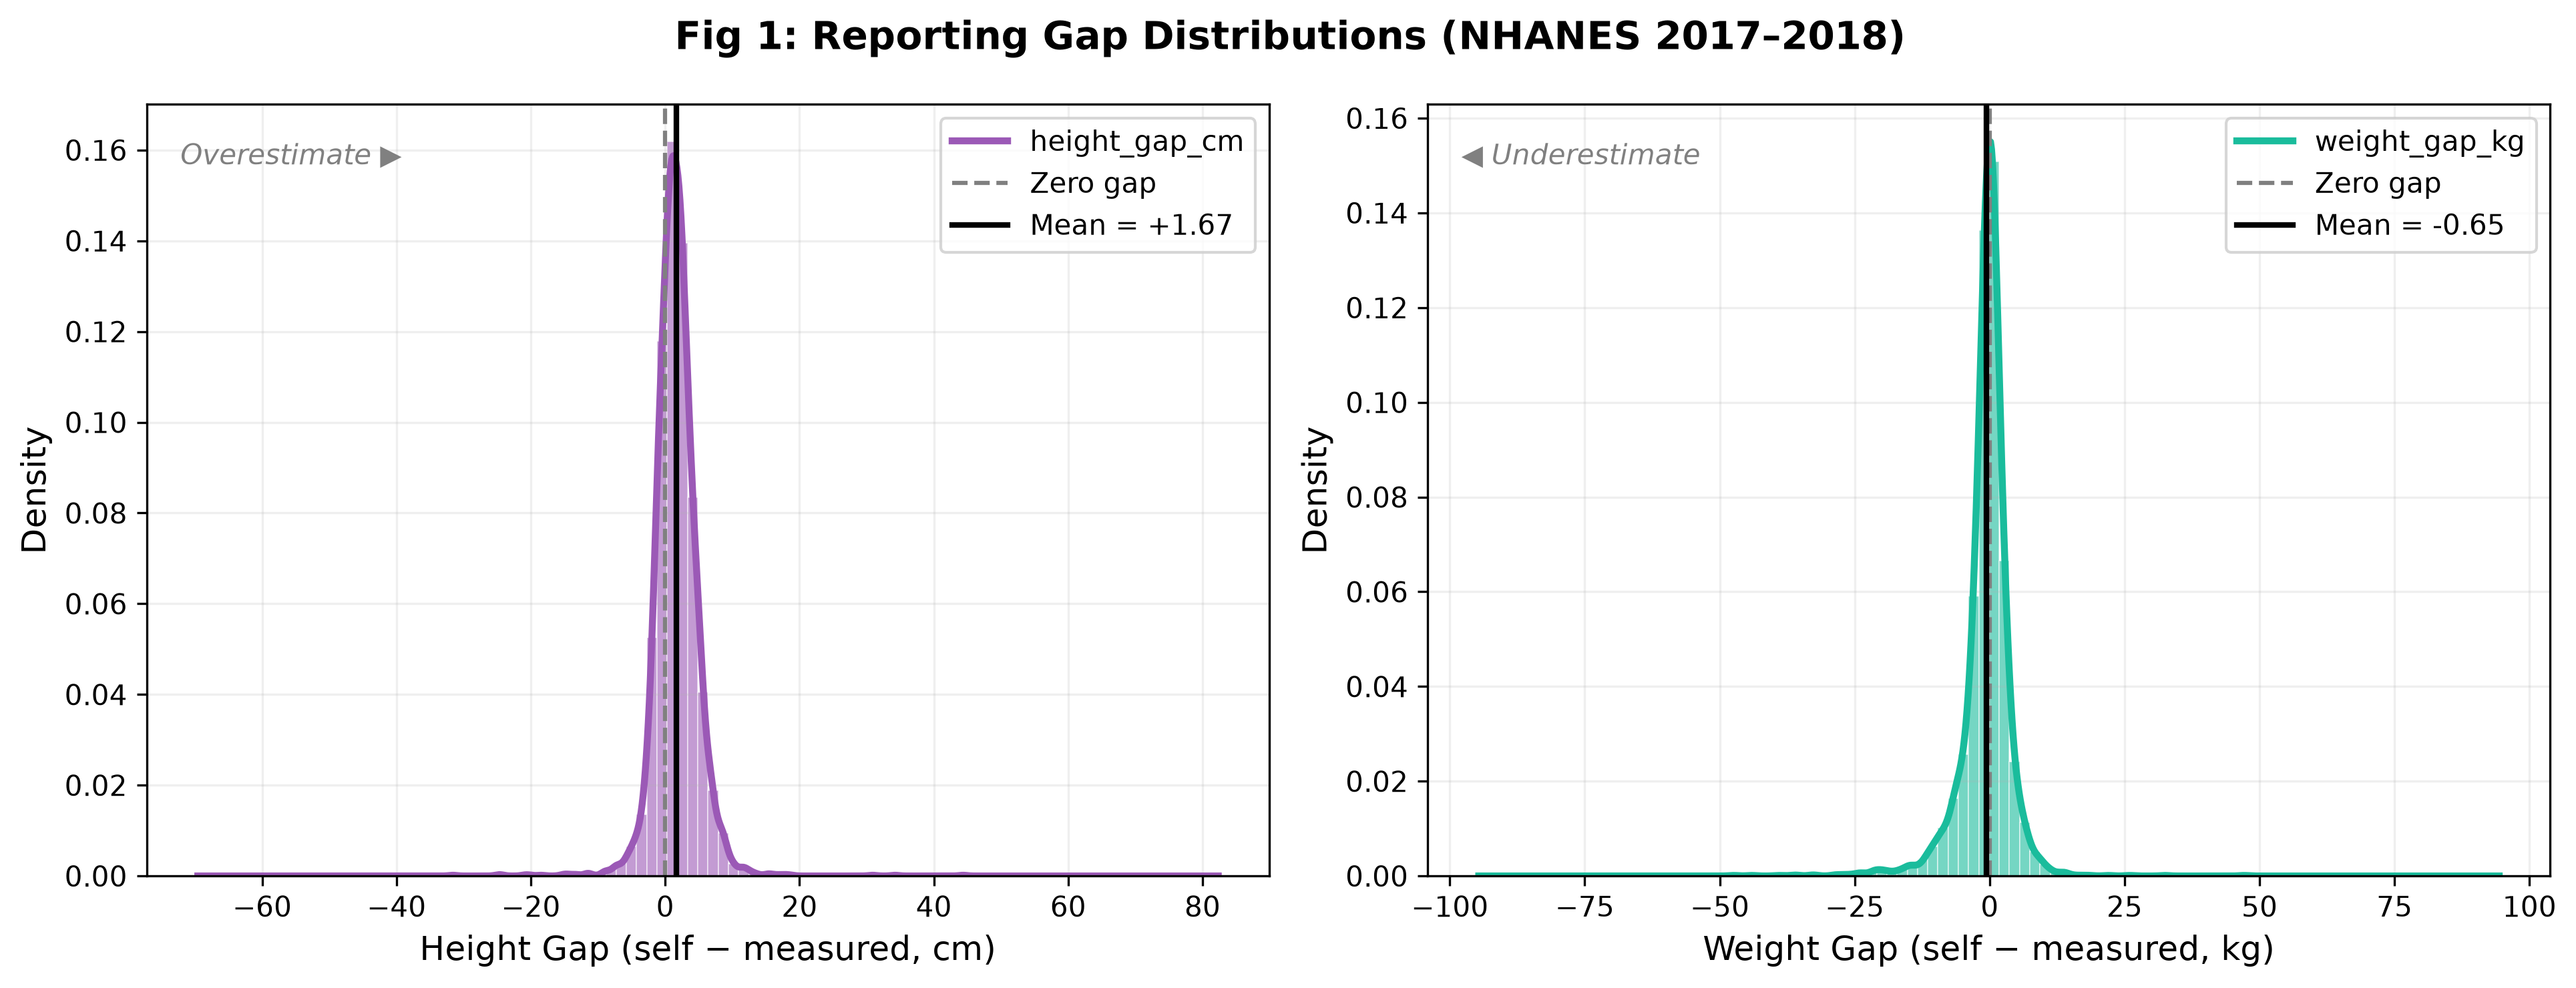
\includegraphics[width=\linewidth]{../results/figures/fig1_reporting_gaps.png}
  \caption{Self-report vs.\ nurse-measured gap distributions (NHANES 2017--2018).
           Height is systematically overestimated; weight is underestimated.}
  \label{fig:gaps}
\end{figure}

In the held-out 2017--2018 data, participants over-report their height
by $+1.69$\,cm on average (SD 3.23\,cm) and under-report their weight by
$-0.67$\,kg (SD 4.84\,kg), closely matching the 2015--2016 development
data ($+1.62$\,cm, SD 3.41; $-0.87$\,kg, SD 4.79). The 95th-percentile
gaps in 2017--2018 (6.88\,cm and 9.32\,kg) are within 0.4\,cm and
0.4\,kg of the development budget used for the attack
(\cref{tab:gap}). Self-reporting behaviour is therefore stable across
cycles, and the lie budget transfers to the held-out data.

\section{Model Performance}

\begin{table}[htbp]
  \centering
  \caption{Model Performance on NHANES 2017–2018 Test Set}
  \label{tab:model_perf}
  \small
  \begin{tabular}{lrrrrrrr}
    \hline
    Config & Input & Model & Accuracy & Precision & Recall & F1 & AUC-ROC \\
    \hline
    measured_rf & measured & RF & 0.7396 & 0.3007 & 0.686 & 0.4181 & 0.7981 \\
    measured_lr & measured & LR & 0.6652 & 0.2569 & 0.7686 & 0.3851 & 0.7734 \\
    reported_rf & reported & RF & 0.7407 & 0.3032 & 0.6942 & 0.4221 & 0.7933 \\
    reported_lr & reported & LR & 0.6685 & 0.2604 & 0.7769 & 0.39 & 0.7796 \\
    \hline
  \end{tabular}
\end{table}

All four models discriminate moderately well (AUC 0.77--0.80) and,
with balanced class weights, detect most diabetic patients (recall
0.69--0.78) at the cost of many false positives (precision 0.26--0.30),
as expected at 13.6\% prevalence. Random Forests are slightly more
accurate than Logistic Regressions. Crucially, Model A (measured
inputs) and Model B (self-reported inputs) perform almost identically
(RF AUC 0.798 vs.\ 0.793; LR 0.773 vs.\ 0.780): using verified inputs
costs nothing in accuracy.

\section{Main Result: Explanation Equivalence}

\begin{figure}[htbp]
  \centering
  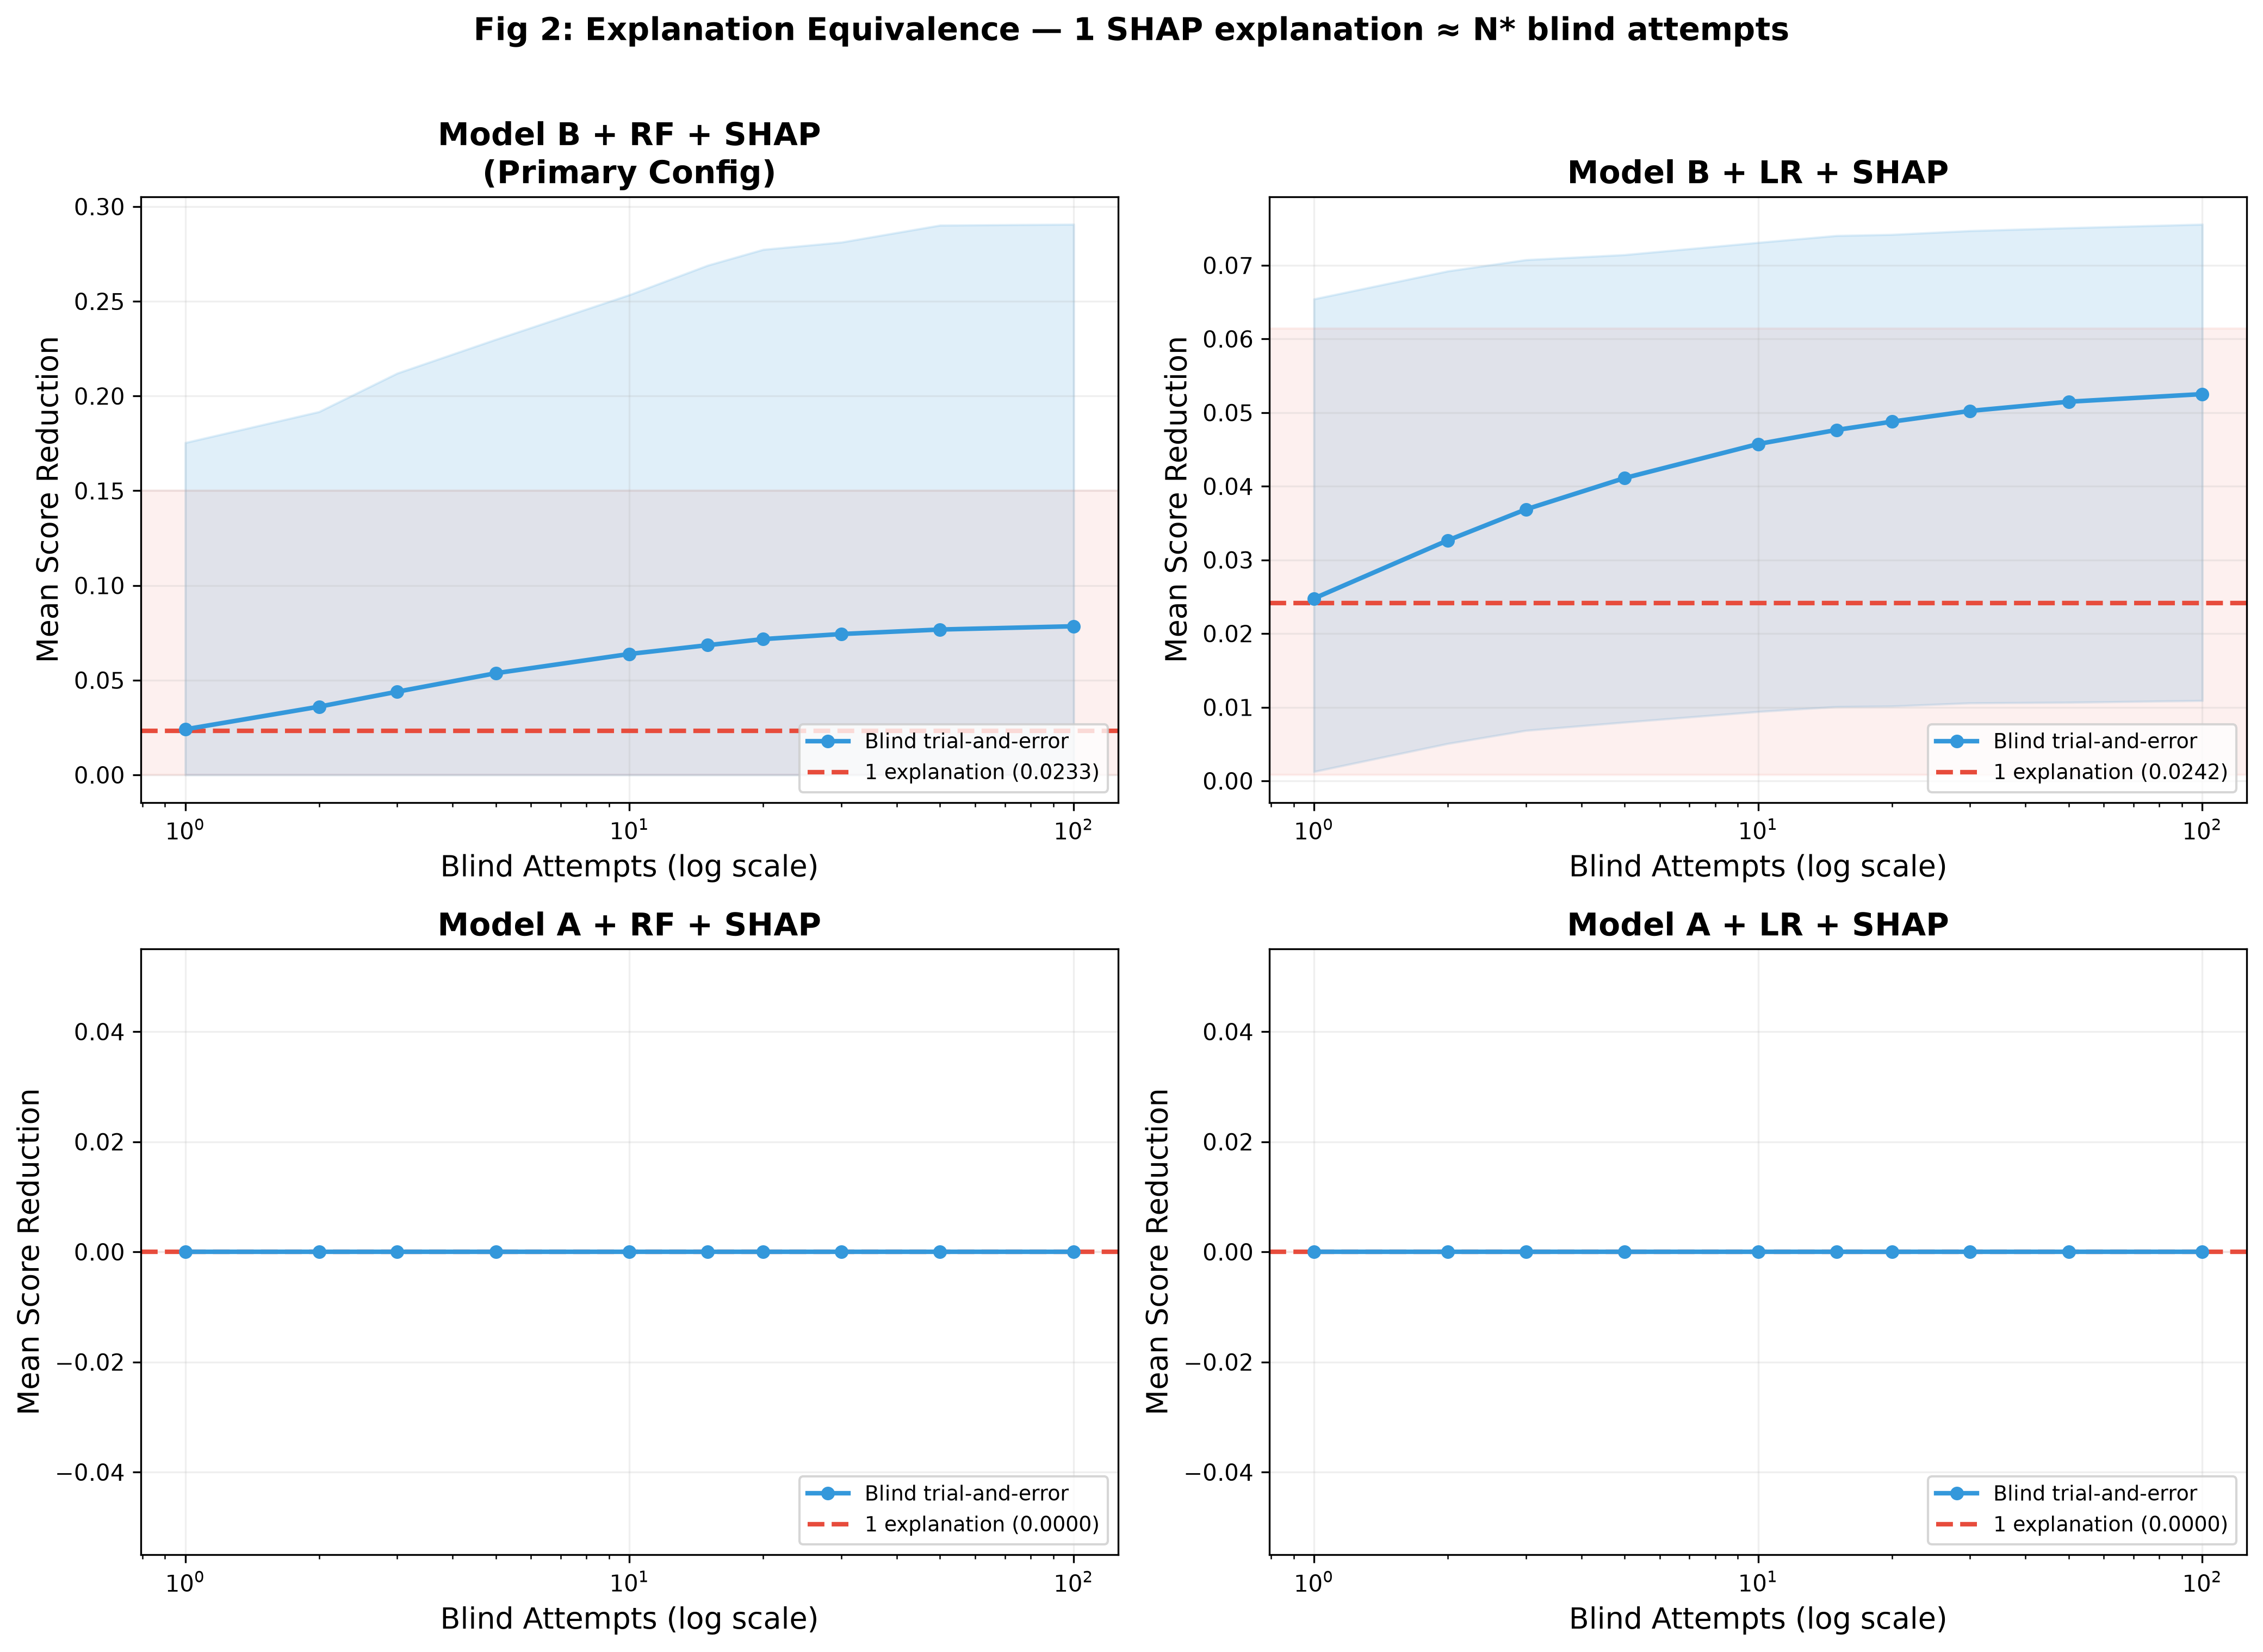
\includegraphics[width=\linewidth]{../results/figures/fig2_main_result.png}
  \caption{Mean score reduction from the best of $N$ blind attempts
           (blue) vs.\ one explanation-guided lie (red dashed), SHAP
           configurations. For Model B the explanation line lies below
           even the first blind attempt, so $N^* = 0$. Model A cannot
           be gamed.}
  \label{fig:main_result}
\end{figure}

\begin{table*}[htbp]
  \centering
  \caption{Main Results: Explanation Equivalence $N^*$ Across All 8 Configurations}
  \label{tab:main_results}
  \small
  \resizebox{\ifdim\width>\linewidth\linewidth\else\width\fi}{!}{%
  \begin{tabular}{lrrrrrrrrr}
    \toprule
    Input & Model & Expl. & N patients & $N^*$ & 95\% CI & Per-patient mean $N^*$ & Per-patient median $N^*$ & \% Useless & \% Worth 10+ \\
    \midrule
    Reported & RF & SHAP & 887 & 0.0 & [0.00, 0.00] & 7.69 & 0.0 & 76.0\% & 8.7\% \\
    Reported & RF & LIME & 887 & 0.0 & [0.00, 0.00] & 7.07 & 0.0 & 73.8\% & 8.1\% \\
    Reported & LR & SHAP & 887 & 0.0 & [0.00, 0.00] & 2.58 & 0.0 & 66.4\% & 5.4\% \\
    Reported & LR & LIME & 887 & 0.0 & [0.00, 0.00] & 2.99 & 0.0 & 56.3\% & 6.1\% \\
    Measured & RF & SHAP & 887 & 0.0 & [0.00, 0.00] & 0.0 & 0.0 & 100.0\% & 0.0\% \\
    Measured & RF & LIME & 887 & 0.0 & [0.00, 0.00] & 0.0 & 0.0 & 100.0\% & 0.0\% \\
    Measured & LR & SHAP & 887 & 0.0 & [0.00, 0.00] & 0.0 & 0.0 & 100.0\% & 0.0\% \\
    Measured & LR & LIME & 887 & 0.0 & [0.00, 0.00] & 0.0 & 0.0 & 100.0\% & 0.0\% \\
    \bottomrule
  \end{tabular}%
  }
\end{table*}


\begin{table*}[htbp]
  \centering
  \caption{Mean risk-score reduction (0-1 scale): one explanation-guided lie vs. the best of N blind lies, and how often the explanation suggested no lie or a lie that raised the risk}
  \label{tab:reductions}
  \small
  \resizebox{\linewidth}{!}{%
  \begin{tabular}{lrrrrrrrr}
    \toprule
    Input & Model & Expl. & 1 explanation & 1 blind & 10 blind & 100 blind & \% no lie suggested & \% lie raised risk \\
    \midrule
    Reported & RF & SHAP & 0.0129 & 0.024 & 0.0638 & 0.0785 & 19.3\% & 23.0\% \\
    Reported & RF & LIME & 0.0117 & 0.024 & 0.0638 & 0.0785 & 3.3\% & 31.1\% \\
    Reported & LR & SHAP & 0.0176 & 0.0248 & 0.0457 & 0.0525 & 31.1\% & 0.0\% \\
    Reported & LR & LIME & 0.0223 & 0.0248 & 0.0457 & 0.0525 & 7.7\% & 0.0\% \\
    Measured & RF & SHAP & 0.0 & 0.0 & 0.0 & 0.0 & 100.0\% & 0.0\% \\
    Measured & RF & LIME & 0.0 & 0.0 & 0.0 & 0.0 & 100.0\% & 0.0\% \\
    Measured & LR & SHAP & 0.0 & 0.0 & 0.0 & 0.0 & 100.0\% & 0.0\% \\
    Measured & LR & LIME & 0.0 & 0.0 & 0.0 & 0.0 & 100.0\% & 0.0\% \\
    \bottomrule
  \end{tabular}%
  }
\end{table*}


These are the \emph{exploratory} 2017--2018 results (v5 code); the
confirmatory 2021--2023 result follows in
\cref{sec:confirmatory-results}. For the primary configuration (Model
B, Random Forest, SHAP) the explanation equivalence is $N^* = 0.0$
(95\% CI: 0.0--1.2), and $N^* = 0.0$ in all eight configurations
(\cref{tab:main_results}). On average, one explanation-guided lie lowers
the risk score by 0.023, while a single blind attempt lowers it by
0.024, the best of 10 attempts by 0.064 and the best of 100 by 0.079
(\cref{tab:reductions}). For the Logistic Regression the picture is the
same (explanation 0.024 with SHAP and 0.022 with LIME, one blind
attempt 0.025). An explanation is therefore worth \emph{about one}
ordinary attempt at the model, and never more.

\subsection*{Why the explanation does not help more}

\begin{enumerate}
  \item \textbf{The explanation only chooses between two features.} With
        realistic lies the direction is fixed (taller, lighter) and the
        size is the same random draw for both strategies, so the
        explanation can add only one piece of information: \emph{which}
        of height and weight to change. A blind patient who tries both
        after two or three attempts has learned the same thing.
  \item \textbf{For the Random Forest, the suggested lie often
        backfires.} 28.5\% (SHAP) and 31.1\% (LIME) of explanation-guided
        lies \emph{raise} the score, and the patient undoes them,
        because a local attribution does not describe how the model
        responds over the whole range of the lie. This is the practical
        face of the impossibility result of
        \citet{bilodeau2024impossibility}. For the Logistic Regression,
        whose response is monotone, no SHAP-guided lie backfires.
\end{enumerate}

\Cref{tab:sensitivity} shows how the two later corrections changed the
primary configuration. Letting the patient undo a bad lie (fix 12) and
reading SHAP relative to the average patient (fix 13) each made the
explanation more useful, but neither lifted it above one blind attempt.

\begin{table}[htbp]
  \centering
  \caption{Primary configuration (Model B, RF + SHAP, 2017--2018) under
           successive code versions. ``1 expl.'' and ``1 blind'' are mean
           score reductions.}
  \label{tab:sensitivity}
  \small
  \begin{tabular}{llrr}
    \toprule
    Code & Headline & 1 expl. & 1 blind \\
    \midrule
    original (pre-registered settings, with bugs) & per-patient mean $N^*$ 12.4 & -- & -- \\
    v3 (fixes 1--11) & $N^* = 0.0$ [0.0, 0.0] & 0.013 & 0.024 \\
    v4 (+ undo a bad lie) & $N^* = 0.0$ [0.0, 0.0] & 0.018 & 0.024 \\
    v5 (+ SHAP read relative to the average) & $N^* = 0.0$ [0.0, 1.2] & 0.023 & 0.024 \\
    \bottomrule
  \end{tabular}
\end{table}

\section{Per-Patient Distribution}

\begin{figure}[htbp]
  \centering
  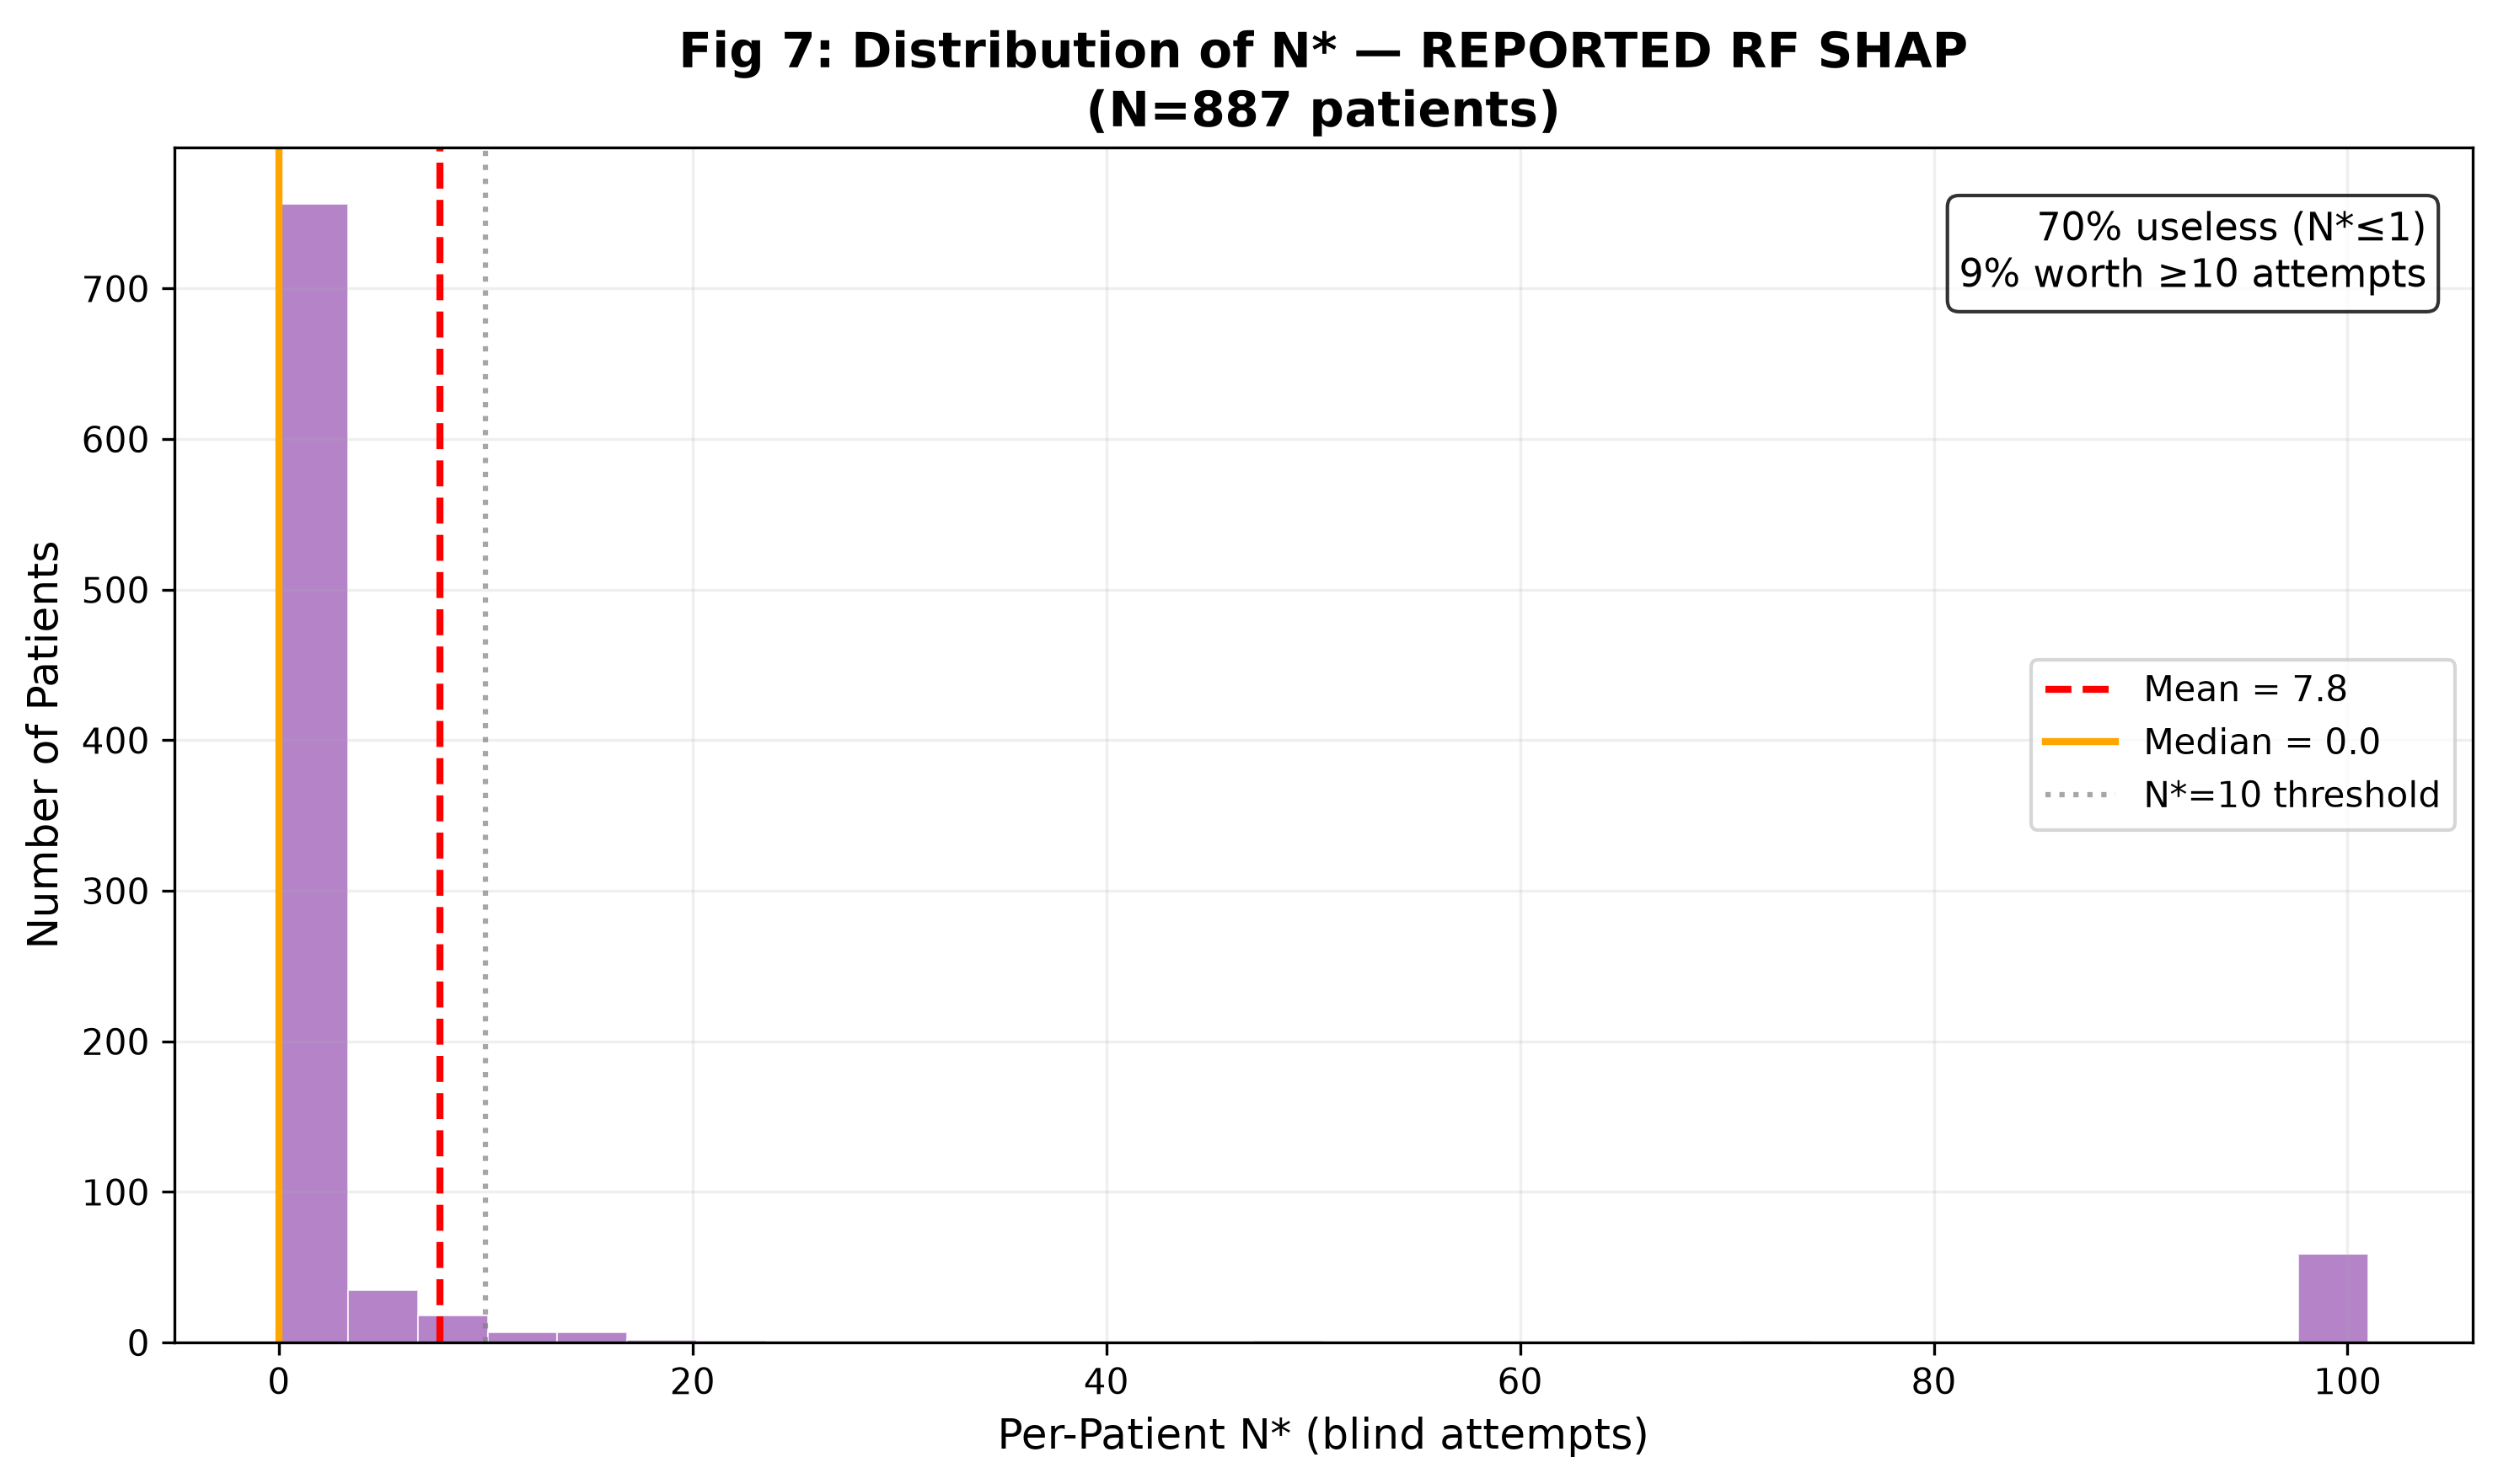
\includegraphics[width=0.85\linewidth]{../results/figures/fig7_nstar_histogram.png}
  \caption{Distribution of per-patient $N^*$ (Model B, RF + SHAP, 887
           patients).}
  \label{fig:hist}
\end{figure}

Per patient (\cref{fig:hist}), the explanation is no better than a
single blind attempt for 69.6\% of patients (RF+SHAP; 52.3\% for
LR+SHAP), and worth 10 or more attempts for 9.5\% (6.4\%); 6.7\% beat
all 100 blind attempts. The distribution is therefore strongly skewed:
a large spike at zero and a thin tail. The per-patient mean $N^*$ (7.8
for RF+SHAP, 3.6 for LR+SHAP) is driven by that tail, which is why the
pre-registered metric averages the reductions over patients first. For
the typical patient, one blind attempt is worth more than the
explanation.

\section{Model A vs.\ Model B}

\begin{figure}[htbp]
  \centering
  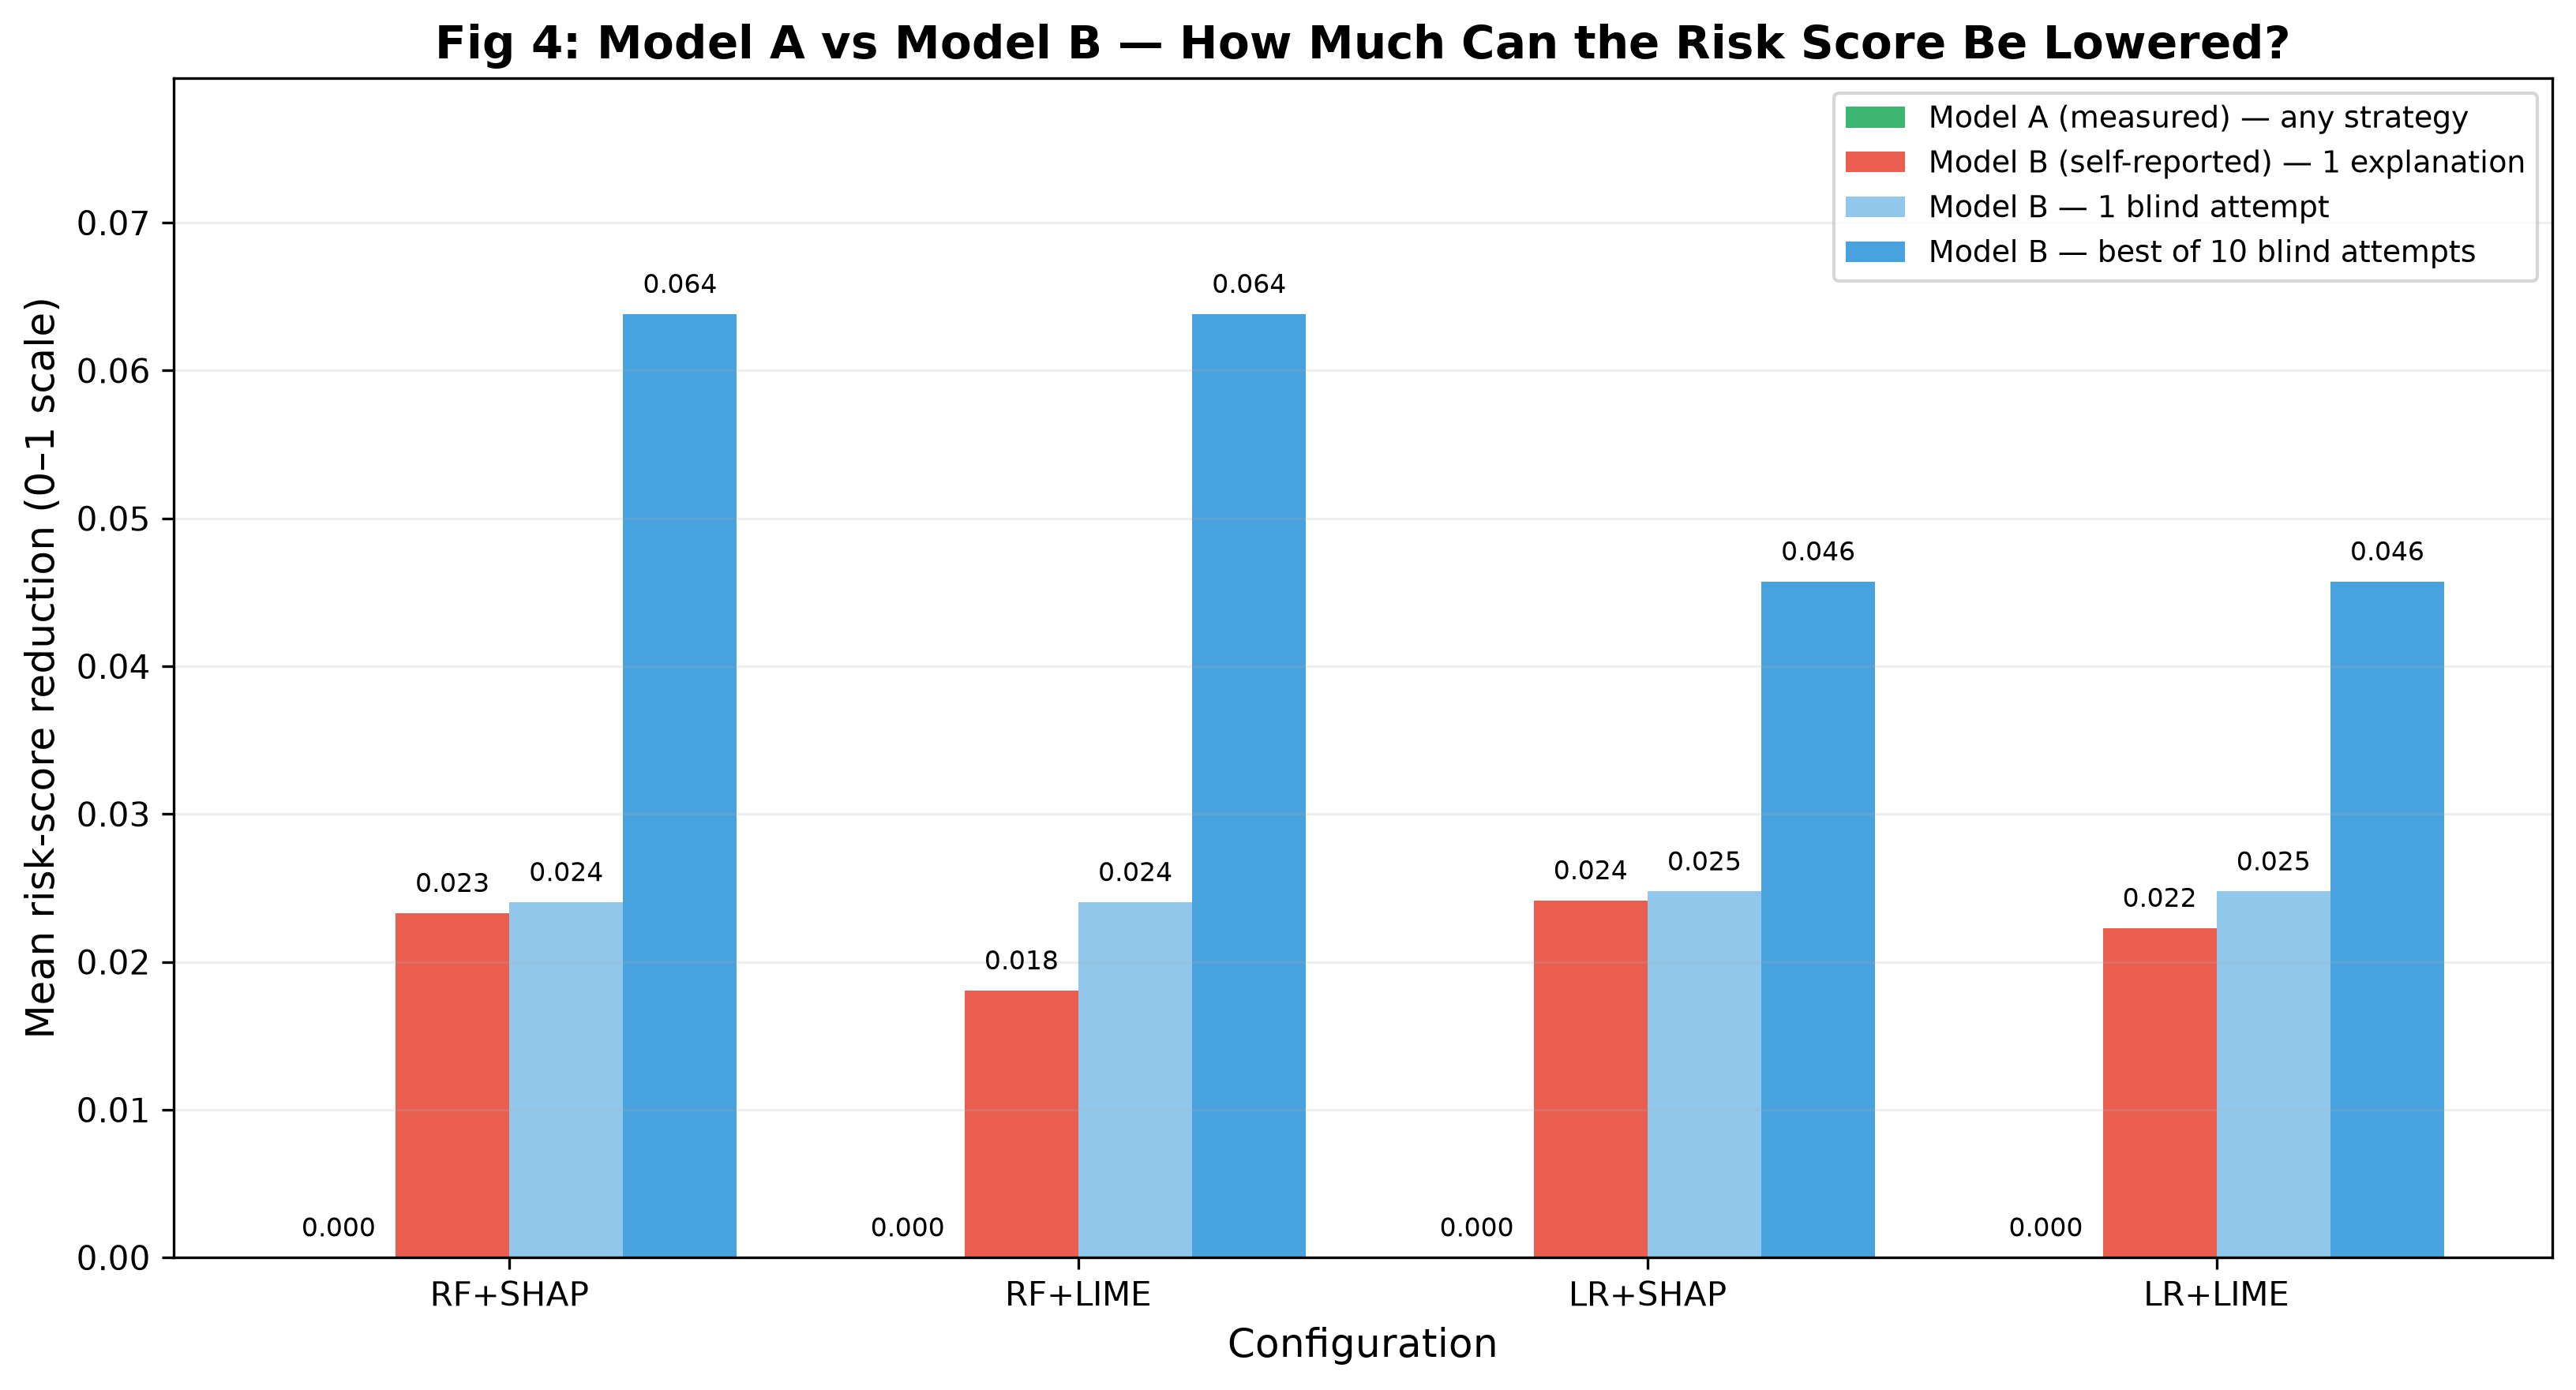
\includegraphics[width=0.95\linewidth]{../results/figures/fig4_model_comparison.png}
  \caption{Mean risk-score reduction for Model A (nurse-measured
           inputs) and Model B (self-reported inputs): one explanation,
           one blind attempt, and the best of 10 blind attempts.}
  \label{fig:modelab}
\end{figure}

\begin{table*}[htbp]
  \centering
  \caption{Model A (Measured) vs Model B (Self-Reported): Vulnerability Comparison}
  \label{tab:model_ab}
  \small
  \resizebox{\ifdim\width>\linewidth\linewidth\else\width\fi}{!}{%
  \begin{tabular}{lrrrrrr}
    \toprule
    Config & Model A $N^*$ & Model B $N^*$ & A: reduction, 10 blind & B: reduction, 1 explanation & B: reduction, 10 blind & B can be gamed \\
    \midrule
    RF+SHAP & 0.0 & 0.0 & 0.0 & 0.0129 & 0.0638 & Yes \\
    RF+LIME & 0.0 & 0.0 & 0.0 & 0.0117 & 0.0638 & Yes \\
    LR+SHAP & 0.0 & 0.0 & 0.0 & 0.0176 & 0.0457 & Yes \\
    LR+LIME & 0.0 & 0.0 & 0.0 & 0.0223 & 0.0457 & Yes \\
    \bottomrule
  \end{tabular}%
  }
\end{table*}


\begin{table*}[htbp]
  \centering
  \caption{Self-reported vs measured height/weight on the same patients: accuracy difference (Model A minus Model B, paired bootstrap 95\% CI) and how far Model B can be gamed. Model A cannot be gamed by construction.}
  \label{tab:input_source}
  \small
  \resizebox{\ifdim\width>\linewidth\linewidth\else\width\fi}{!}{%
  \begin{tabular}{lrrrrr}
    \toprule
    Model & AUC A (measured) & AUC B (self-reported) & Difference A-B & 95\% CI (paired bootstrap) & B: max reduction, 10 blind lies \\
    \midrule
    RF & 0.7981 & 0.7933 & 0.0047 & [-0.0093, +0.0177] & 0.0638 \\
    LR & 0.7734 & 0.7796 & -0.0062 & [-0.0127, +0.0002] & 0.0457 \\
    \bottomrule
  \end{tabular}%
  }
\end{table*}


That Model A cannot be gamed is true \emph{by design}, not an
experimental finding: its height and weight come from the nurse, so
there is nothing the patient can lie about, and its zeros in
\cref{tab:model_ab} follow from the threat model. The comparison
therefore has two measurable parts. First, how far Model B, which
differs only in using the self-reported values, can be gamed: by
0.046--0.064 with ten blind attempts and 0.053--0.079 with a hundred.
Second, what it costs to use measured instead of self-reported inputs
(\cref{tab:input_source}): on the same 887 test patients, the AUC
difference (Model A minus Model B) is $+0.005$ for the Random Forest
(95\% CI $-0.009$ to $+0.018$) and $-0.006$ for the Logistic Regression
($-0.013$ to $+0.000$), both indistinguishable from zero.
\textbf{Verifying two inputs removes the attack surface at no
measurable cost in accuracy.}

\section{SHAP vs.\ LIME Agreement}

\begin{figure}[htbp]
  \centering
  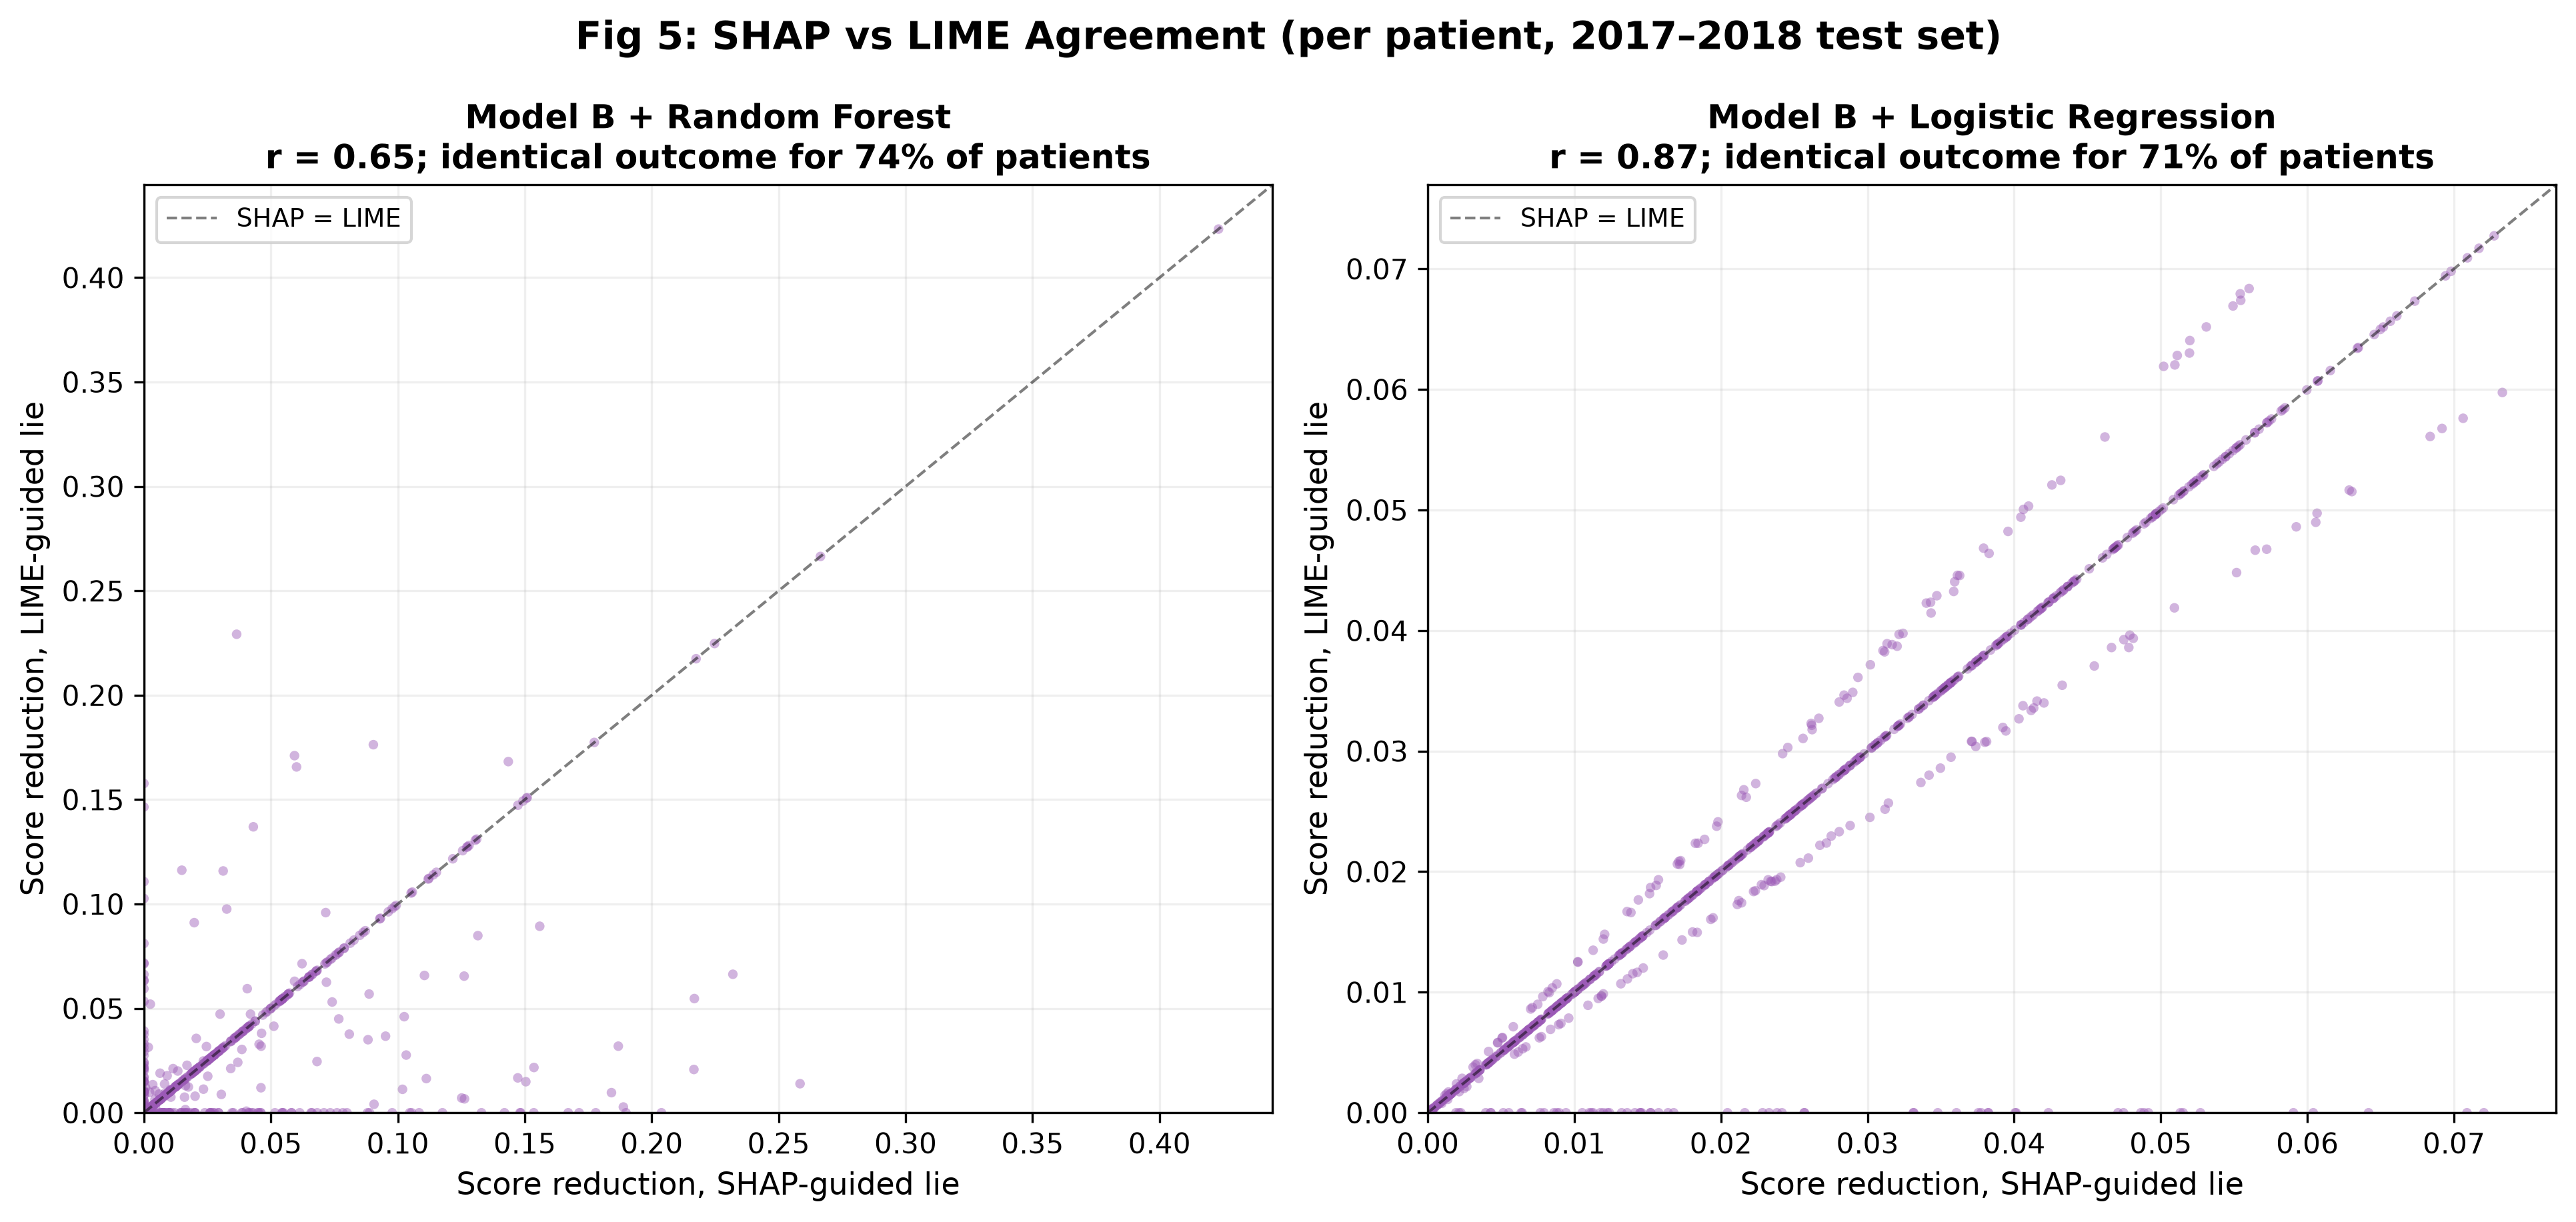
\includegraphics[width=\linewidth]{../results/figures/fig5_shap_lime_scatter.png}
  \caption{Per-patient score reduction from the SHAP-guided lie vs.\
           the LIME-guided lie (Model B). Points on the diagonal: both
           explanations led to the same outcome.}
  \label{fig:scatter}
\end{figure}

Because each patient receives the same lie size under SHAP and LIME,
differences come only from the explanation (\cref{fig:scatter}). The
two methods lead to the same outcome for 74\% of patients with the
Random Forest and 71\% with the Logistic Regression; the per-patient
correlation is $r = 0.65$ and $0.87$. At the configuration level they
agree: both give $N^* = 0$, and SHAP is slightly better than LIME
(Random Forest 0.023 vs.\ 0.018; Logistic Regression 0.024 vs.\
0.022). The two methods sometimes point
to different features or directions for the same patient, but neither
helps more than a blind attempt.

\section{Statistical Tests}

\begin{table}[htbp]
  \centering
  \caption{Statistical Tests: Explanation vs Blind (N=10), Wilcoxon Signed-Rank}
  \label{tab:stats}
  \small
  \begin{tabular}{lrrr}
    \toprule
    Config & Wilcoxon p & Cohen's d & Significant \\
    \midrule
    reported\_rf\_shap & 1.000000 & -0.801 & No \\
    reported\_rf\_lime & 1.000000 & -0.789 & No \\
    reported\_lr\_shap & 1.000000 & -1.336 & No \\
    reported\_lr\_lime & 1.000000 & -1.238 & No \\
    measured\_rf\_shap & 1.000000 & 0.000 & No \\
    measured\_rf\_lime & 1.000000 & 0.000 & No \\
    measured\_lr\_shap & 1.000000 & 0.000 & No \\
    measured\_lr\_lime & 1.000000 & 0.000 & No \\
    \bottomrule
  \end{tabular}
\end{table}


The pre-registered one-sided Wilcoxon signed-rank test of
\emph{explanation $>$ blind at $N=10$} is not significant in any
configuration ($p = 1.0$, also after Holm correction across the eight
configurations; \cref{tab:stats}). For Model B the effect sizes are
large and \emph{negative} (Cohen's $d$ from $-0.66$ to $-1.24$): ten
blind attempts lower the score clearly more than one explanation. For
Model A all reductions are zero and there is nothing to test.

\section{Comparison Dataset: CDC Diabetes Health Indicators}

\begin{table*}[t]
  \centering
  \caption{Comparison dataset (CDC Diabetes Health Indicators, UCI 891; BRFSS 2015, 1{,}000 sampled test respondents): one explanation vs.\ blind attempts, with self-reported BMI as the only gameable feature.}
  \label{tab:uci891}
  \small
  \resizebox{\linewidth}{!}{%
  \begin{tabular}{llrrrrrrrrrrr}
    \toprule
    Model & Expl. & N & N* & N* 95\% CI & 1 explanation & 1 blind & 10 blind & Per-patient mean N* & \% useless & \% lie undone & Wilcoxon p & Cohen's d \\
    \midrule
    RF & SHAP & 1000 & 0.0 & [0.00, 1.04] & 0.0409 & 0.0436 & 0.0772 & 16.98 & 67.8 & 16.5 & 1.0 & -0.703 \\
    RF & LIME & 1000 & 0.0 & [0.00, 0.00] & 0.0324 & 0.0436 & 0.0772 & 13.86 & 74.7 & 13.6 & 1.0 & -0.829 \\
    LR & SHAP & 1000 & 0.0 & [0.00, 1.12] & 0.0369 & 0.0373 & 0.0655 & 4.04 & 49.8 & 0.0 & 1.0 & -1.142 \\
    LR & LIME & 1000 & 0.0 & [0.00, 0.00] & 0.0257 & 0.0373 & 0.0655 & 2.85 & 63.8 & 0.0 & 1.0 & -1.316 \\
    \bottomrule
  \end{tabular}}
\end{table*}


On 1,000 sampled test respondents of the BRFSS 2015 survey, with
self-reported BMI as the only gameable feature, the result is the same
(\cref{tab:uci891}): $N^* = 0.0$ in all four configurations (upper CI
bound at most 1.1), one explanation-guided lie lowers the score by
0.026--0.041 against 0.037--0.044 for one blind attempt, and no
Wilcoxon test is significant. The finding is therefore not specific to
NHANES or to the height/weight pair. The comparison is limited: BRFSS
has no measured BMI (so no Model~A), its diabetes label is
self-reported, and the BMI lie budget had to be borrowed from NHANES.

\section{Configuration Overview}

\begin{figure}[htbp]
  \centering
  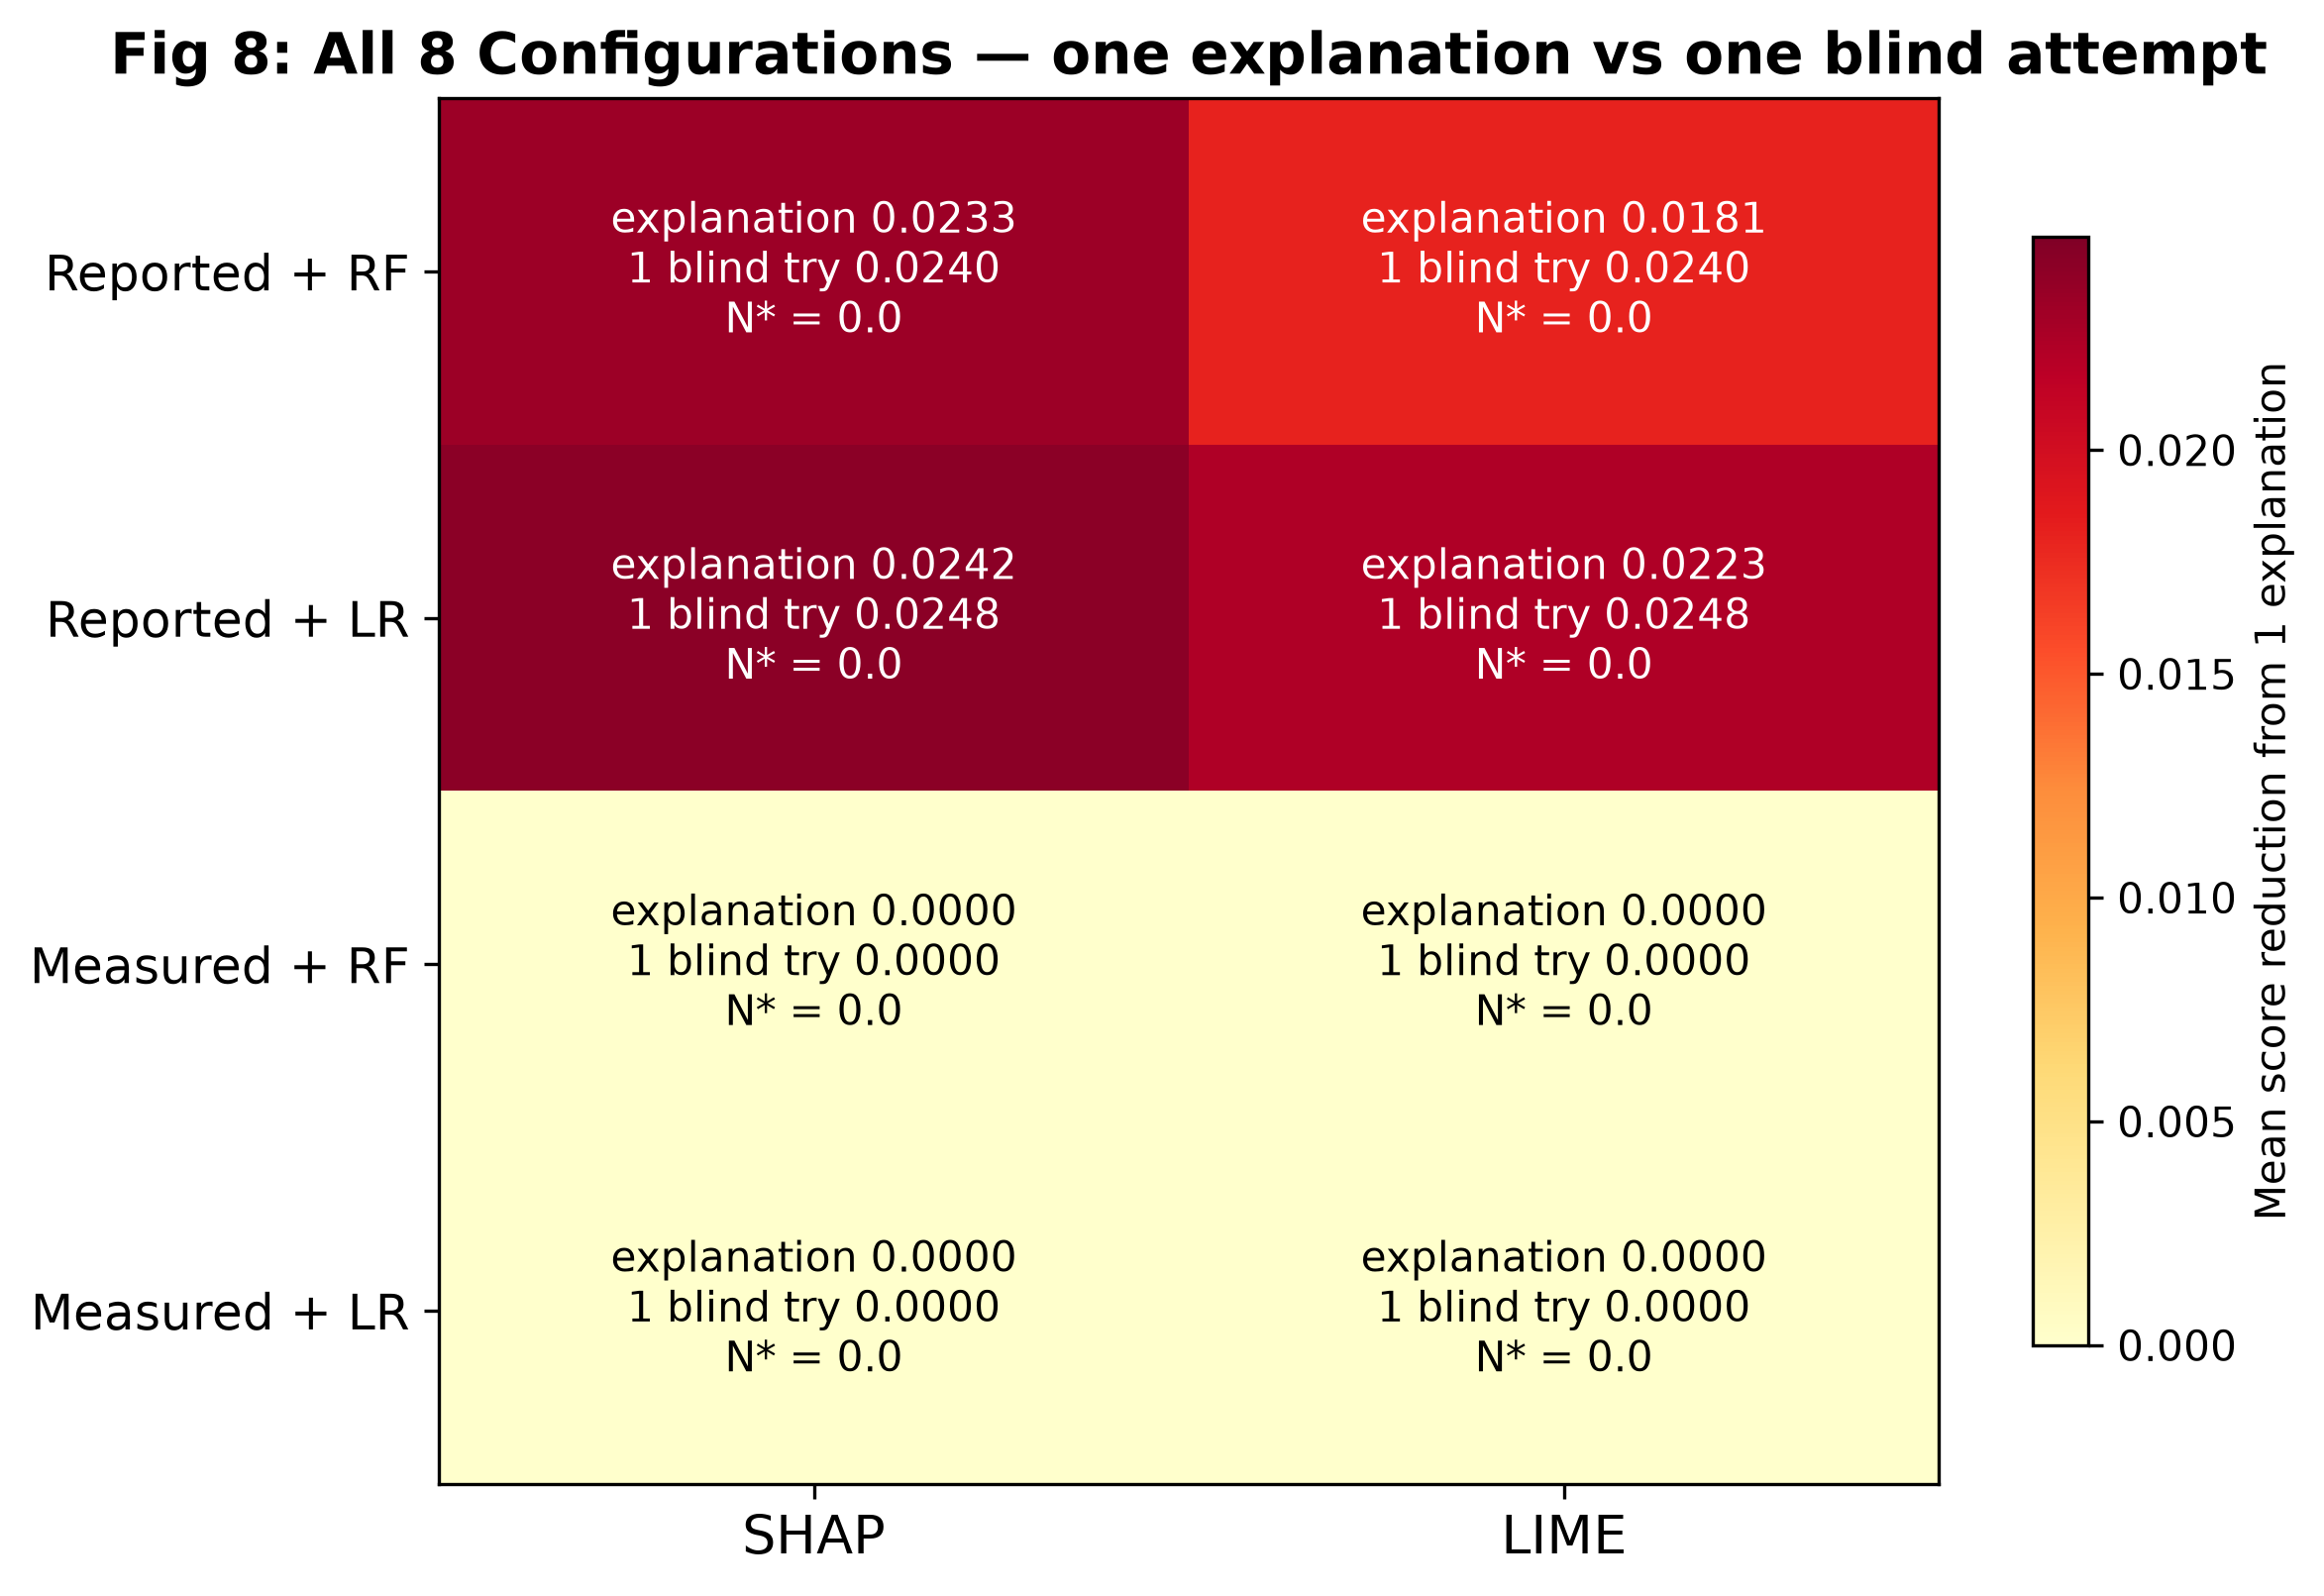
\includegraphics[width=0.8\linewidth]{../results/figures/fig8_config_heatmap.png}
  \caption{All 8 configurations: mean score reduction from one
           explanation (colour), one blind attempt, and $N^*$.}
  \label{fig:heatmap}
\end{figure}

\Cref{fig:heatmap} summarises all eight configurations. In every
Model~B cell, one explanation lowers the score by at most as much as
one blind attempt. The explanation does relatively best for the
Logistic Regression, whose response to a lie is monotone, and worst for
the Random Forest with LIME, where explanation-guided lies most often
backfire. Model~A cells are zero throughout.

\section{Confirmatory Result: NHANES 2021--2023}
\label{sec:confirmatory-results}

The confirmatory run used the code and settings fixed at the
\texttt{v0.2-preregistration} tag (commit \texttt{5b2f240}), unchanged,
on NHANES August 2021--August 2023: 5{,}628 adults with complete data
(11.9\% with diabetes) and 1{,}126 test patients.  The reporting gap was
again stable (height $+1.73$\,cm, weight $-0.65$\,kg on average;
95th percentiles 6.84\,cm and 9.04\,kg against the 7.28\,cm and
8.96\,kg budget used).

\begin{table}[htbp]
  \centering
  \caption{Confirmatory result, NHANES 2021--2023 (pre-registered,
           $n = 1{,}126$ test patients). Mean score reductions; Model A
           (measured) is 0 in every column by design.}
  \label{tab:confirmatory}
  \small
  \begin{tabular}{lrcrrrr}
    \toprule
    Model B config & $N^*$ & 95\% CI & 1 expl. & 1 blind & 10 blind & Cohen's $d$ \\
    \midrule
    RF + SHAP (primary) & 1.42 & [1.21, 1.62] & 0.034 & 0.028 & 0.070 & $-0.71$ \\
    RF + LIME & 0.00 & [0.00, 0.00] & 0.024 & 0.028 & 0.070 & $-0.76$ \\
    LR + SHAP & 1.07 & [0.00, 1.20] & 0.035 & 0.035 & 0.062 & $-1.14$ \\
    LR + LIME & 0.00 & [0.00, 0.00] & 0.032 & 0.035 & 0.062 & $-1.19$ \\
    \bottomrule
  \end{tabular}
\end{table}

For the primary configuration, $N^* = 1.42$ (95\% CI 1.21--1.62): one
SHAP explanation is worth about one and a half blind attempts, inside
the pre-registered ``minimal advantage'' band ($N^* < 5$), and the
upper confidence bound is far below 5 (\cref{tab:confirmatory}).
Across Model~B, $N^*$ ranges from 0 to 1.42; the one-sided Wilcoxon
test of explanation $>$ ten blind attempts is not significant in any
configuration ($p = 1.0$, also after Holm correction), with large
negative effect sizes.  Every pre-registered prediction held.  As in
2017--2018, Random Forest lies suggested by an explanation backfired
for 27\% of patients.  Unlike 2017--2018, SHAP now does slightly
\emph{better} than one blind attempt (0.034 vs.\ 0.028 for the Random
Forest), which is why $N^*$ is above zero; LIME does not.

Model~A again cannot be gamed.  The accuracy difference between
measured and self-reported inputs on the same test patients is $+0.006$
for the Random Forest (95\% CI $-0.014$ to $+0.026$) and $-0.012$ for
the Logistic Regression ($-0.023$ to $-0.002$), i.e.\ in this cycle the
self-reported Logistic Regression is slightly \emph{more} accurate.
Either way the difference is about one hundredth of AUC, small against
the 0.06--0.07 by which ten blind lies lower a Model~B score.

% ============================================================
% CHAPTER 6 — DISCUSSION
% ============================================================
\chapter{Discussion}
\label{chap:discussion}

\section{Interpretation of Results}

Based on our pre-registered interpretation guide:
\begin{description}
  \item[$N^* < 5$:] Explanations offer minimal advantage. Restricting
       them does not meaningfully reduce gaming risk; the benefit of
       transparency outweighs the gaming concern.
  \item[$5 \leq N^* \leq 20$:] Explanations offer moderate advantage.
       Design-level countermeasures (e.g., rate limiting, input noise)
       are worth considering.
  \item[$N^* > 20$:] Explanations are powerful attack vectors.
       Restricting or anonymising them may be warranted; input
       verification is the more robust safeguard.
\end{description}

Our confirmatory result of $N^* = 1.42$ (95\% CI 1.21--1.62) for the
primary configuration, and at most 1.42 in any configuration, falls in
the \textbf{low threat} category ($N^* < 5$), as pre-registered. Under
realistic lies, an explanation gives a patient no better route to a
lower score than trying one or two answers. This runs against the intuition that explanations are
``instructions for cheating''. The reason is that a feature attribution
answers ``what contributed to this score?'', not ``what should I
change?'', and the two can point in different directions.

\section{Policy Implications}

\begin{itemize}
  \item \textbf{Withholding explanations is not an effective safeguard.}
        It would take information away from honest patients and
        clinicians while barely slowing a motivated patient, who can
        do better by trial and error.
  \item \textbf{Verify the inputs that drive the prediction.} The
        vulnerability lies in the self-reported values: the model
        using nurse-measured height and weight cannot be gamed and is
        just as accurate.
  \item \textbf{Present attributions as contributions, not advice.}
        Since attributions often do not indicate a profitable change,
        explanation interfaces should not suggest that they do.
\end{itemize}

\section{Limitations}

\begin{itemize}
  \item \textbf{Domain:} Results are specific to diabetes risk
        prediction from self-reported anthropometrics (NHANES, and BRFSS
        as a comparison whose diabetes label is itself self-reported).
  \item \textbf{Survey changes:} In 2021--2023 blood pressure is
        measured oscillometrically and the activity question was
        redesigned; both were mapped before the data was seen.
  \item \textbf{Explanation's room to help:} With the direction of a
        realistic lie fixed and its size random, an explanation can
        only choose which of two features to change; a richer lie model
        could give it more room.
  \item \textbf{Model of the patient:} We model one way of reading an
        explanation (follow the top realistic suggestion once). A more
        sophisticated reader, or a counterfactual explanation, could
        extract more.
  \item \textbf{Single-feature, single-step adversary:} Real adversaries
        may adjust several features or iterate.
  \item \textbf{Lie model:} Lie sizes are uniform within the
        95th-percentile gap, in the observed direction. Using the
        maximum lie or allowing either direction is a one-line change
        (\cref{tab:deviations}); that sensitivity analysis is future work.
  \item \textbf{Static model:} The model does not adapt to gaming.
  \item \textbf{Pre-registration:} The plan was recorded as a git tag in
        the project repository rather than in an independent registry;
        a first run on the 2017--2018 data was seen before the analysis
        was corrected, and eight settings deviate from the first plan
        (\cref{sec:deviations}). We therefore treat 2017--2018 as
        exploratory and rest the conclusion on the re-registered
        2021--2023 test.
\end{itemize}

\section{Comparison with Prior Work}

\citet{slack2020fooling} showed that a dishonest \emph{provider} can make
SHAP and LIME hide a model's behaviour; we study the opposite direction,
an honest model whose explanations might help a \emph{patient}, and find
that they help less than trial and error. \citet{shokri2021privacy} and
\citet{milli2019model} showed that explanations leak information about
the training data and the model, so that a few explanation queries can
replace many ordinary ones for reconstructing a model; our results show
that this does not carry over to a patient lowering their own score
under realistic lies. \citet{ghalme2021strategic} found that hiding the
decision rule usually does not help the decision-maker; our empirical
result points the same way for explanations. Finally,
\citet{bilodeau2024impossibility} proved that feature attributions can
fail to predict how a model responds to a change; our experiment
measures how large this failure is in a realistic clinical setting and
shows that it is large enough to keep explanations from being much
more useful for gaming than a blind attempt. What we add is an equal-cost blind baseline, a lie model
measured from real human misreporting, and a matched pair of models
that isolates input verification.

% ============================================================
% CHAPTER 7 — CONCLUSION AND FUTURE WORK
% ============================================================
\chapter{Conclusion and Future Work}
\label{chap:conclusion}

\section{Summary of Findings}

This thesis introduced \textit{explanation equivalence} ($N^*$), a metric
for quantifying the gaming advantage conferred by an XAI explanation over
blind trial-and-error. Applied to a diabetes risk model trained on NHANES
data, our pre-registered confirmatory test on unseen NHANES 2021--2023
data found $N^* = 1.42$ (95\% CI 1.21--1.62) for the primary
configuration and at most 1.42 overall: one SHAP or LIME explanation is
worth about one to two blind attempts. This places the threat in the
\textbf{low} zone, as predicted, and the exploratory 2017--2018 analysis
and the BRFSS comparison agree. For the Random Forest, explanation-guided
lies often raised the score instead. The model using nurse-measured
inputs could not be gamed, with no meaningful loss of accuracy.

The key policy finding is: \textbf{withholding explanations is not an
effective safeguard against gaming; verifying self-reported inputs is.}

\section{Contributions}

\begin{enumerate}
  \item \textbf{New metric:} Explanation equivalence $N^*$.
  \item \textbf{Empirical lie budget:} Grounded in real NHANES data.
  \item \textbf{Matched models:} Two models differing only in measured vs.\
        self-reported inputs, isolating the effect of input verification.
  \item \textbf{Pre-registered study:} A confirmatory test on unseen
        data under a public pre-registration (\texttt{v0.2}); the first
        plan's compromised test set, the corrections and all deviations
        are disclosed.
  \item \textbf{Hand-checked pipeline and replication:} A closed-form
        check of the code on UCI Heart Disease, and a replication on the
        CDC Diabetes Health Indicators survey.
  \item \textbf{Open code:} Full pipeline released at \url{https://github.com/AkkiNikumbh/BTECH_PROJECT}.
\end{enumerate}

\section{Future Work}

\begin{itemize}
  \item \textbf{Sensitivity analysis:} Repeat the experiment with the
        maximum lie and with lies in either direction (settings already
        available in the code).
  \item \textbf{Multi-feature attacks:} Allow the adversary to simultaneously
        adjust multiple features within a combined budget.
  \item \textbf{Adaptive defences:} Study adversarially robust training as
        a complement to input verification.
  \item \textbf{Other domains:} Apply the $N^*$ framework to credit scoring,
        hiring, or recidivism prediction.
  \item \textbf{Other explanation methods:} Evaluate counterfactual
        explanations, integrated gradients, and attention maps.
  \item \textbf{Human subjects:} Measure actual gaming behaviour in a user
        study, where participants attempt to lower their predicted risk.
\end{itemize}

% ============================================================
% APPENDICES
% ============================================================
\appendix

\chapter{NHANES Column Mapping}
\label{app:columns}

% NHANES column mapping (LaTeX version of docs/column_mapping.md),
% included by thesis/main.tex, Appendix A.

\Cref{tab:columns} lists the NHANES variables used in this project, their
source, and whether a patient could change them (``gameable'').  Only
\texttt{WHD010} and \texttt{WHD020} are attacked in the experiment;
\texttt{SMQ020} and \texttt{PAQ650} are self-reported yes/no answers that
could in principle be flipped, but are not attacked because no
reported-vs-measured gap exists to bound such a lie.

\begin{longtable}{p{2.1cm}p{6.0cm}p{1.9cm}p{3.5cm}}
  \caption{NHANES columns, sources and gameability.}
  \label{tab:columns}\\
  \toprule
  Column & Description & Gameable? & Reason \\
  \midrule
  \endfirsthead
  \toprule
  Column & Description & Gameable? & Reason \\
  \midrule
  \endhead
  \bottomrule
  \endfoot
  \texttt{SEQN}     & Respondent sequence number (patient ID) & -- & Identifier \\
  \texttt{RIDAGEYR} & Age in years at screening & No & Verified by ID \\
  \texttt{RIAGENDR} & Gender (1 = male, 2 = female) & No & Recorded by staff \\
  \texttt{BMXHT}    & \textbf{Measured} standing height (cm), nurse & No & Nurse measures directly \\
  \texttt{BMXWT}    & \textbf{Measured} body weight (kg), nurse & No & Nurse measures directly \\
  \texttt{WHD010}   & \textbf{Self-reported} height (inches; $\times 2.54$ to cm); valid 47--84, missing codes 7777/9999 & \textbf{Yes} & Patient reports verbally; bounded by the reported-vs-measured gap \\
  \texttt{WHD020}   & \textbf{Self-reported} weight (pounds; $\times 0.453592$ to kg); valid 75--600, missing codes 7777/9999 & \textbf{Yes} & Patient reports verbally; bounded by the reported-vs-measured gap \\
  \texttt{LBXGH}    & Glycohaemoglobin HbA1c (\%) --- \textbf{diabetes target} ($\geq 6.5\%$) & No & Laboratory blood test \\
  \texttt{BPXSY1}   & Systolic blood pressure, first reading (mmHg) & No & Measured by staff \\
  \texttt{SMQ020}   & Smoked at least 100 cigarettes in life (1 = yes, 2 = no; missing 7/9) & Maybe & Binary self-report (not attacked) \\
  \texttt{PAQ650}   & Vigorous recreational activity (1 = yes, 2 = no; missing 7/9) & Maybe & Binary self-report (not attacked) \\
\end{longtable}

The two feature sets use \texttt{RIDAGEYR}, \texttt{RIAGENDR},
\texttt{BPXSY1}, \texttt{SMQ020}, \texttt{PAQ650} plus either the
measured pair (\texttt{BMXHT}, \texttt{BMXWT}; Model A) or the
self-reported pair (\texttt{WHD010}, \texttt{WHD020}; Model B).


\chapter{Full Statistical Tables}
\label{app:stats}

\section{Reporting Gap Comparison}
\begin{table}[htbp]
  \centering
  \caption{Reporting Gap Comparison: 2015--2016 vs 2017--2018}
  \label{tab:gap}
  \small
  \begin{tabular}{lrrrr}
    \hline
    Feature & Dev mean direction & Dev 95th pct budget & Holdout 95th pct & Absolute change \\
    \hline
    Height & positive & 7.28 cm & 6.88 cm & 0.40 cm \\
    Weight & negative & 8.96 kg & 9.32 kg & 0.36 kg \\
    \hline
  \end{tabular}
\end{table}

\section{Model A vs.\ Model B}
See \cref{tab:model_ab} in \cref{chap:results}.

\chapter{Additional Figures}
\label{app:figures}

\begin{figure}[htbp]
  \centering
  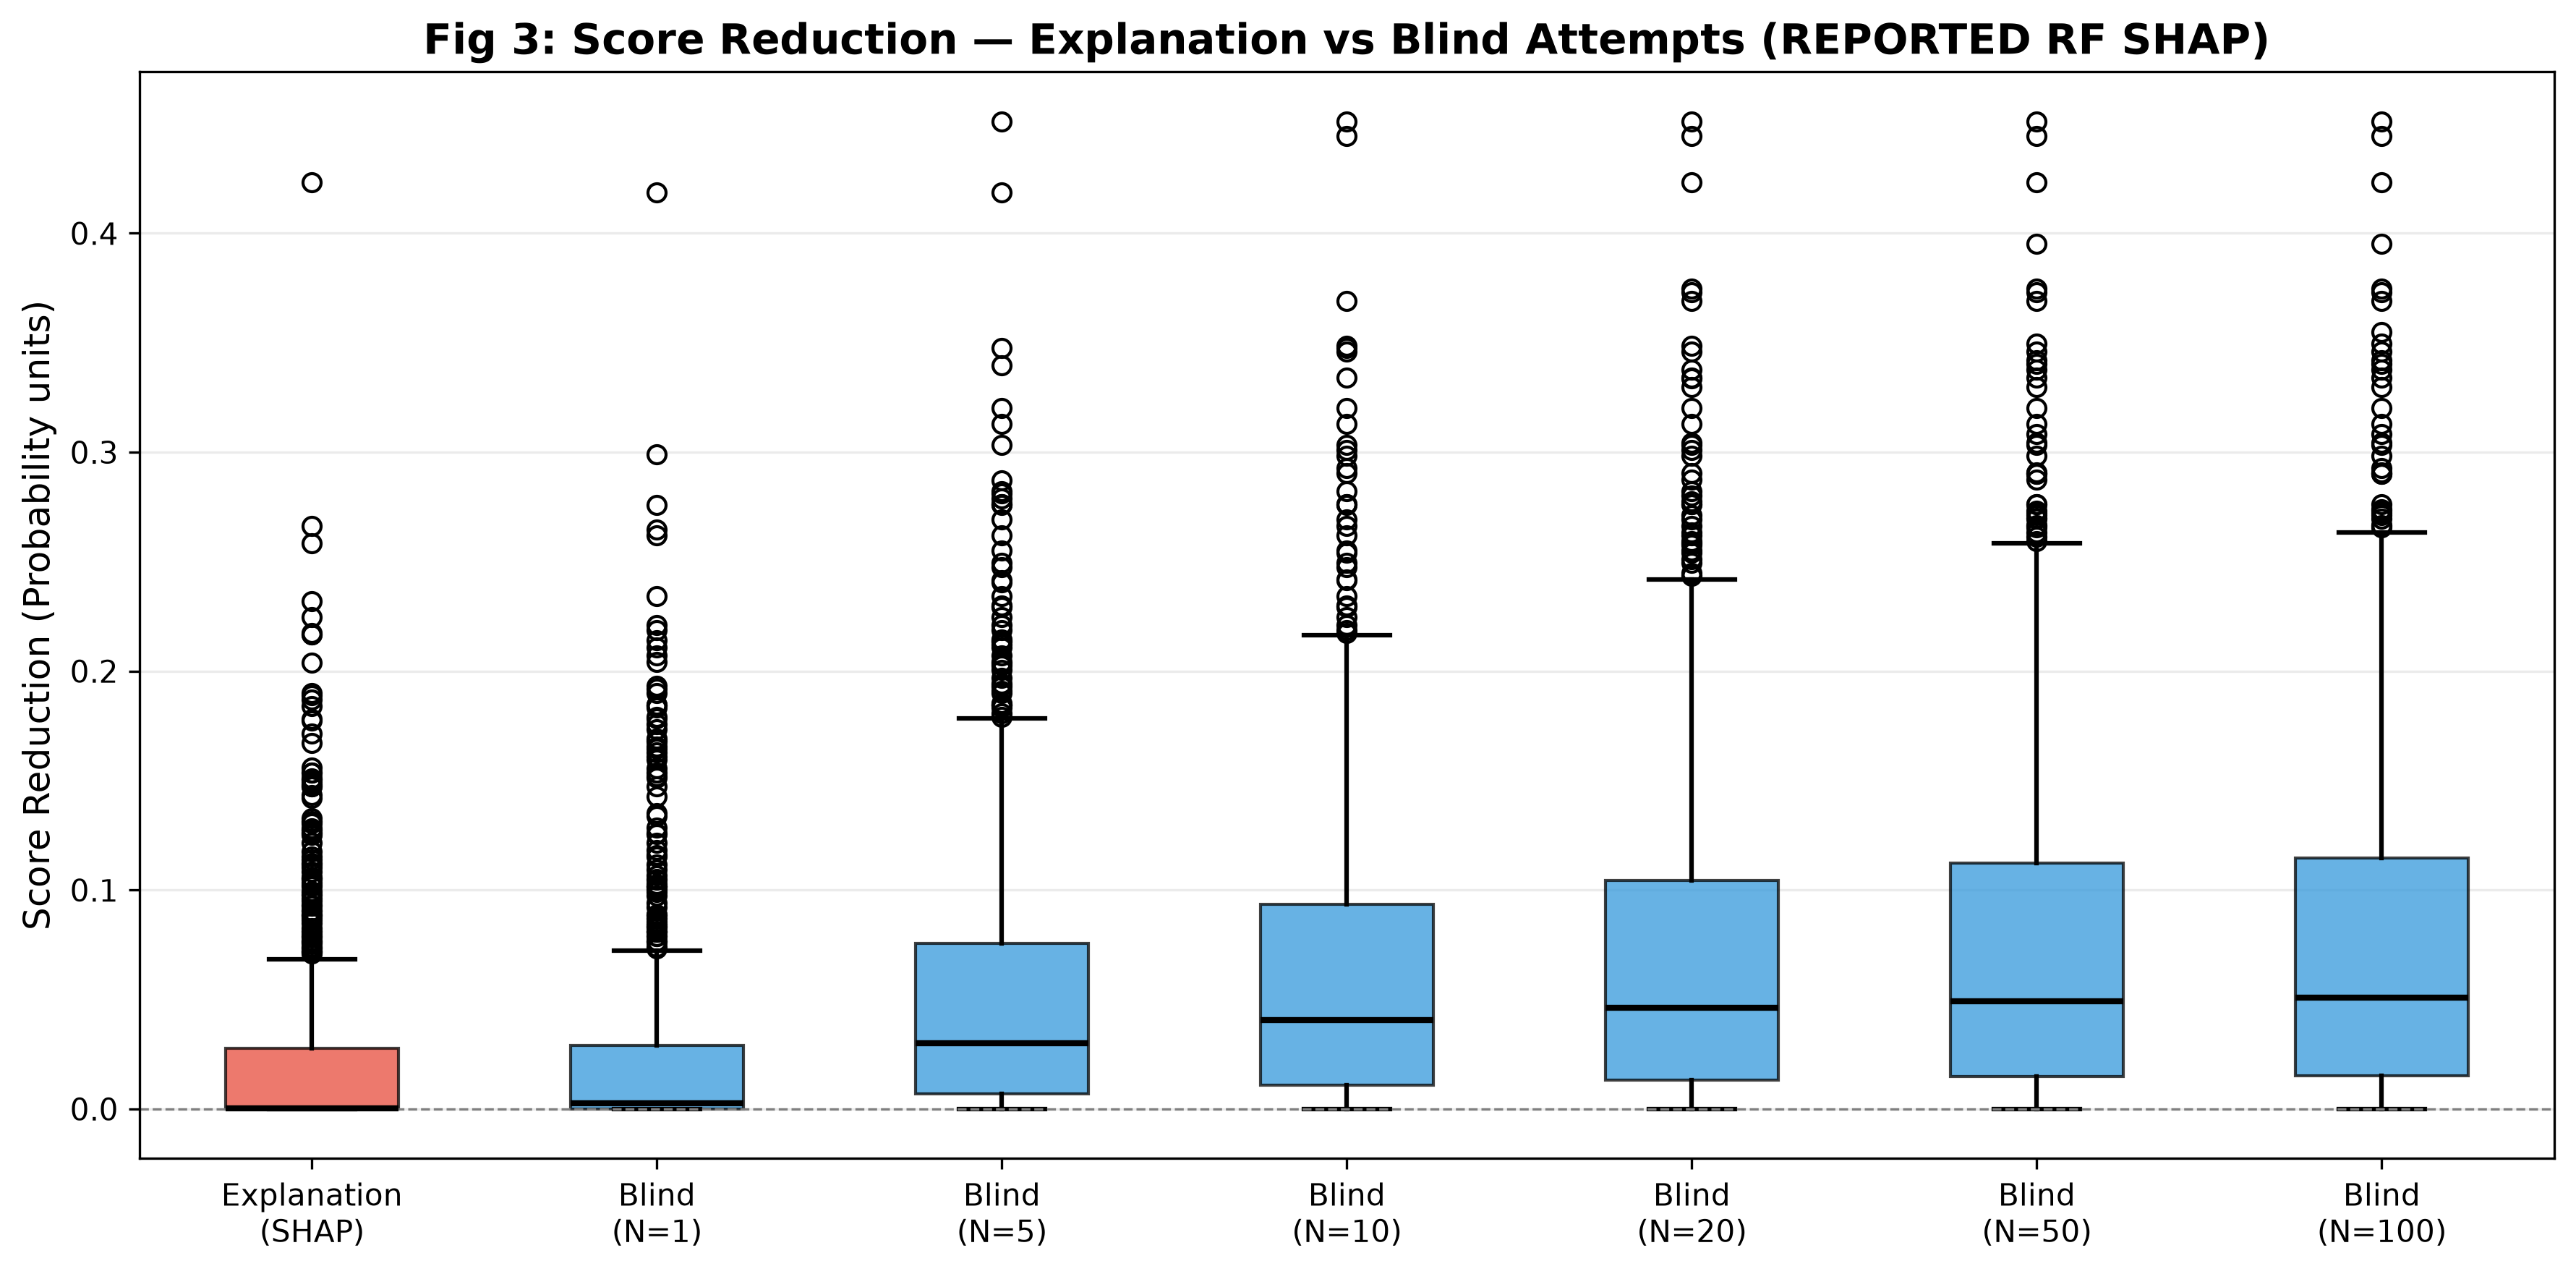
\includegraphics[width=0.85\linewidth]{../results/figures/fig3_score_reductions.png}
  \caption{Score reduction box plots for the primary configuration
           (Model B, RF + SHAP). Red box = one explanation; blue boxes =
           best of $N$ blind attempts.}
  \label{fig:boxplots}
\end{figure}

\begin{figure}[htbp]
  \centering
  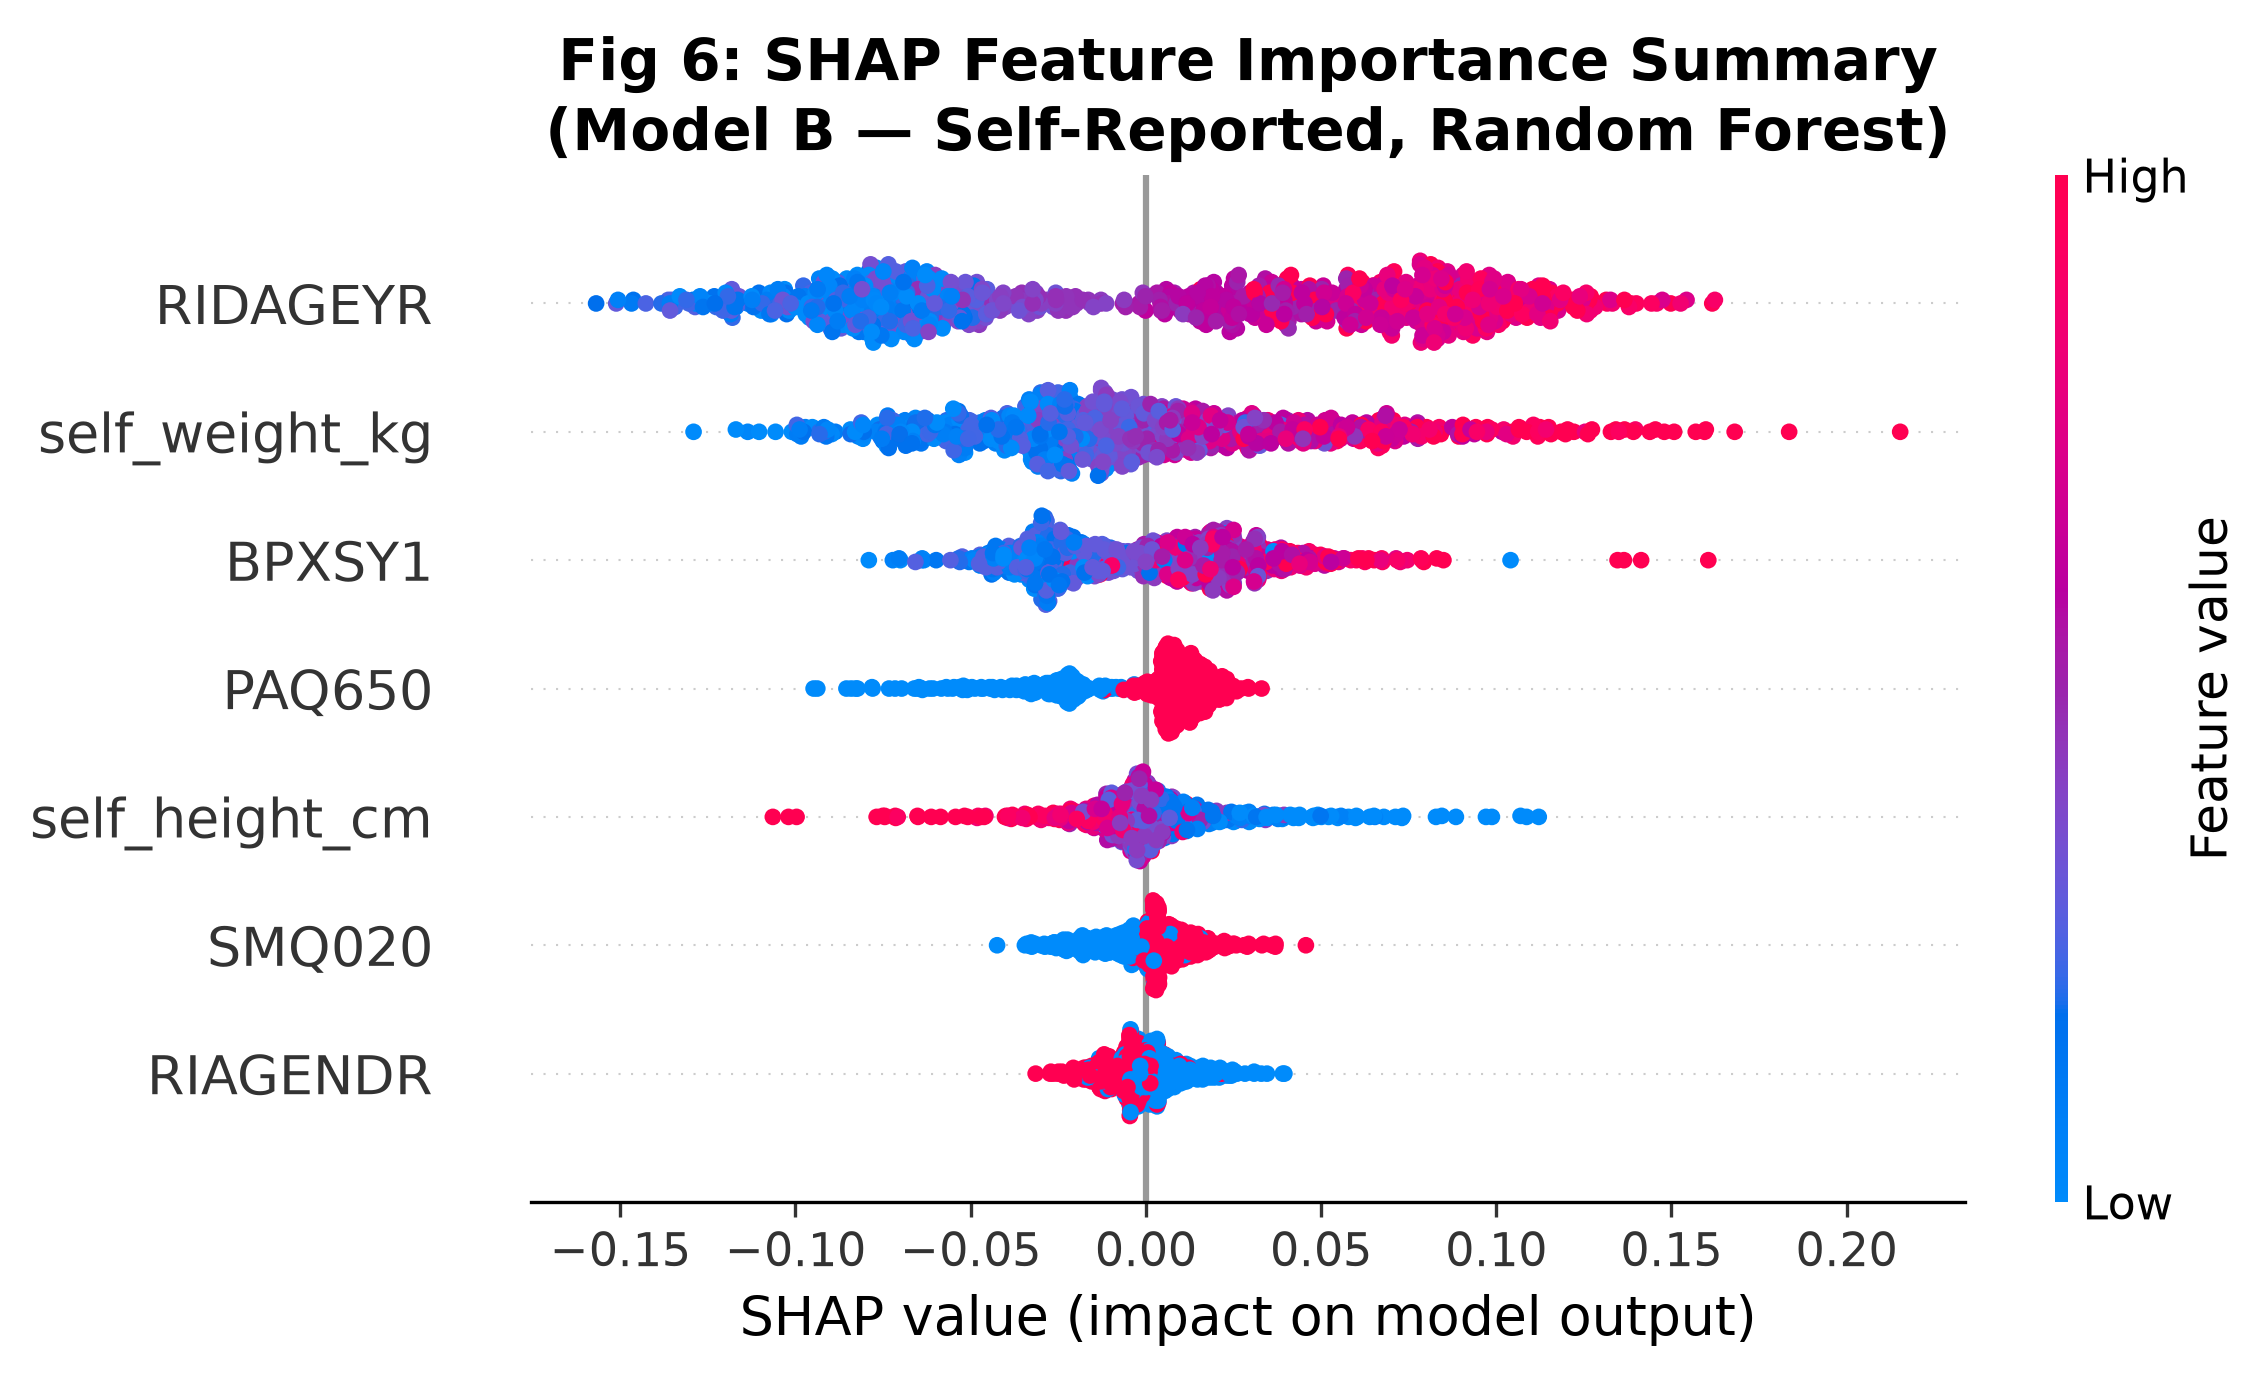
\includegraphics[width=0.85\linewidth]{../results/figures/fig6_shap_summary.png}
  \caption{SHAP feature importance summary (Model B, Random Forest).
           Each dot is a patient; colour shows feature value.}
  \label{fig:shap_summary}
\end{figure}

\chapter{Code Repository}
\label{app:code}

\section{Repository Structure}
\begin{lstlisting}[language=bash]
BTP/
  src/                # Core Python modules
    config.py         # Seeds, paths, FINAL_CONFIG
    data_loader.py    # NHANES loading & preprocessing
    gap_analysis.py   # Self-reporting error analysis
    models.py         # DiabetesModel class
    explanations.py   # ExplanationGenerator (SHAP+LIME)
    adversarial.py    # AdversarialSimulator
    metrics.py        # N* computation, CI, Wilcoxon
    visualization.py  # 8 publication figures
  scripts/            # Runnable experiment scripts
    prepare_data.py   # Stage 3: data preparation
    run_trial.py      # Stage 5: trial run
    run_final.py      # Stage 7: final experiment
    run_analysis.py   # Stage 8: figures + tables
    review_stage*.py  # Per-stage verification
  paper/              # LaTeX paper source
  docs/               # Column mapping, analysis plan
  results/            # Generated figures and tables
  data/               # Raw XPT files + processed pickles
  tests/              # pytest test suite (40 tests)
\end{lstlisting}

\section{Installation and Execution}
\begin{lstlisting}
# 1. Install dependencies
pip install -r requirements.txt

# 2. Download NHANES data
python scripts/download_nhanes.py

# 3. Prepare data (Stage 3)
python scripts/prepare_data.py

# 4. Run final experiment (Stage 7, ~35 minutes)
python scripts/run_final.py

# 5. Generate figures and tables (Stage 8)
python scripts/run_analysis.py

# 6. Compile paper / thesis (requires LaTeX)
cd paper  && pdflatex main && bibtex main && pdflatex main && pdflatex main
cd thesis && pdflatex main && bibtex main && pdflatex main && pdflatex main
\end{lstlisting}

% ============================================================
% REFERENCES
% ============================================================
\bibliographystyle{plainnat}
\bibliography{../paper/references}

\end{document}
